\documentclass[t]{beamer}

\usepackage[czech]{babel}
\usepackage[utf8]{inputenc}
\usepackage[T1]{fontenc}
\usepackage{csquotes}
\usepackage{expl3,biblatex}
\addbibresource{main.bib}
\usepackage[bottom]{footmisc}
\usepackage{booktabs}
\usefonttheme[onlymath]{serif}
\usetheme[
  workplace=c4e,
]{MU}
\usepackage{tikz}
\usepackage[absolute,overlay]{textpos}
\setlength{\TPHorizModule}{1cm}
\setlength{\TPVertModule}{1cm}
\newcommand<>{\fullsizegraphic}[1]{%
  \begin{textblock}{0}(0,0)%
    \only#2{%
      \begin{tikzpicture}%
        \fill [black] (current page.north west) rectangle (current page.south east);
        \node[overlay] at (current page.center)
          {\includegraphics[keepaspectratio,width=\paperwidth,height=\paperheight]{#1}};
      \end{tikzpicture}%
    }%
  \end{textblock}%
}
\usepackage{hyperref}
\usepackage{multimedia}
\usepackage{animate}

\usepackage{textcomp}
\usepackage{graphicx} % Required for inserting images %potřebuje David
\usepackage{gensymb} %for degrees %potřebuje David




\title[Wanted: Shadows]{Wanted: Shadows}
\subtitle[Alternativní název prezentace]{aneb zjišťování výšky mraků pomocí Coralu a RaspberryPi}
\author[AstroX]{M. Matta, E. Plic, T. Rajchman, D. Němec, L. Kohoutková\texorpdfstring{\\}{, }astrox@mgplzen.cz}
\institute[C4e]{Tým AstroX z Masarykovo Gymnázia}
\date{\today}
\subject{Předmět prezentace}
\keywords{klíčová, slova, prezentace}
\begin{document}

\begin{frame}[plain]
\maketitle
\end{frame}

\section[Úvod]{Dlouhý název sekce 1}
\subsection[Osnova]{Dlouhý název podsekce 1}
\begin{frame}{Osnova}
\begin{itemize}
    \item Kdo jsme?
    \item V čem soutěžíme?
    \item Jak jsme na soutěž přišli?
    \item Co jsme vymysleli?
    \item Jak jsem se dostali na FAV?
    \item Co jsme naprogramovali?
    \item Co se stane, až to doběhne?
    \item Poděkování
    \item Zdroje
\end{itemize}
    
\end{frame}

\subsection[Poděkování]{Dlouhý název podsekce 1}
\begin{frame}[c]
\begin{center}
\color{mubeamer@base}
\Huge \textbf{Poděkování}
\end{center}
\end{frame}

\subsection[Kdo jsme?]{Dlouhý název podsekce 1}
\begin{frame}{Kdo jsme?}
\begin{columns}[T]
    \begin{column}{.6\textwidth}
    \hspace{2mm} \textbf{Středoškoláci z Masarykova gymnázia}
    \vspace{2mm}
        \begin{itemize}
            \setlength\itemsep{2mm}
            \item Lucie Kohoutková
            \item Matyáš Matta
            \item David Němec
            \item Eduard Plic
            \item Tomáš Rajchman
        \end{itemize}
    \end{column}
    \begin{column}{.4\textwidth}
    \includegraphics[width=4.5cm]{images/Logo_Masaryk.png}
    \end{column}
\end{columns}


\vspace{-0.5cm}
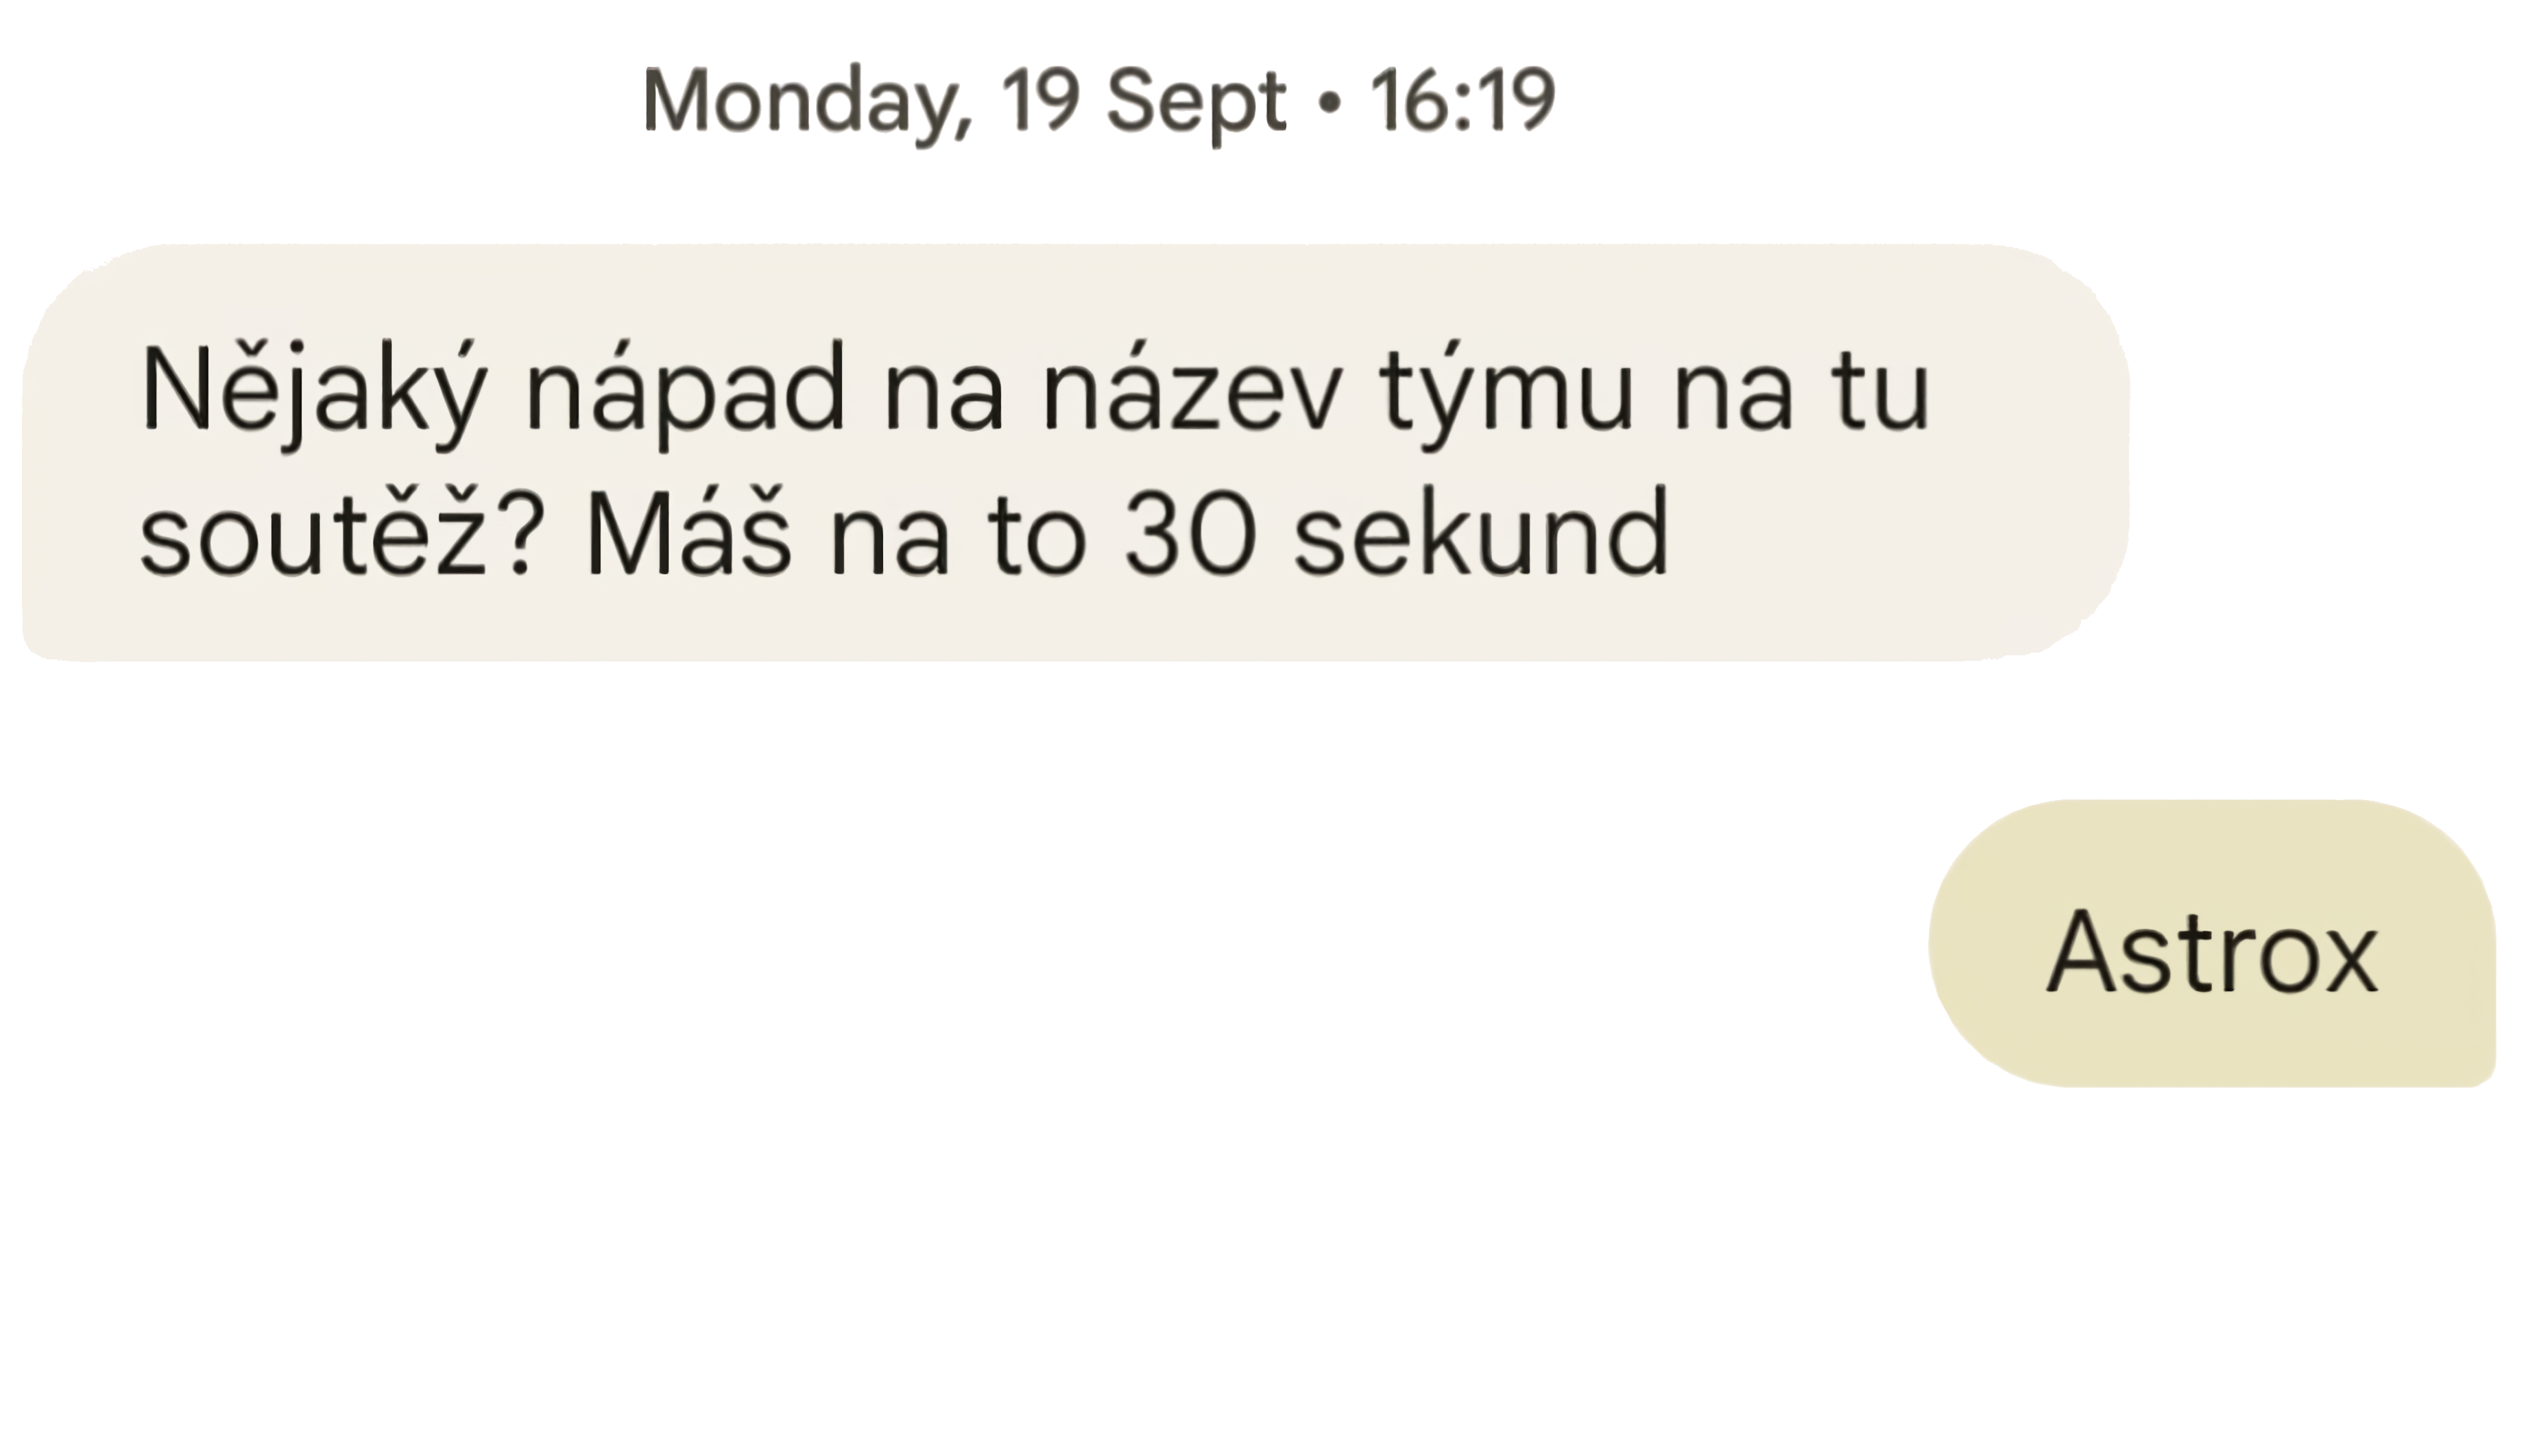
\includegraphics[height=3cm]{images/messages2.png}
    
\end{frame}

\section[O soutěži]{Dlouhý název sekce 1}
\subsection[V čem soutěžíme?]{Dlouhý název podsekce 1}
\begin{frame}{V čem soutěžíme?}
  \begin{columns}[T]
    \begin{column}{.4\textwidth}
    
\includegraphics[width=5cm]{images/AstroPi_key_visual_pillars.png}
    \end{column}
    \begin{column}{.6\textwidth}
    \begin{itemize}
        \item mezinárodní soutěž Astro Pi pořádaná \alert{Evropskou vesmírnou agenturou}
        \item mise Space Lab, která umožňuje týmům mladých studentů provést vlastní experiment na \alert{ISS}
        \item programování mikropočítače Raspberry Pi programem napsaným v \alert{Pythonu}
    \end{itemize}
    \end{column}
  \end{columns}
    
\end{frame}

\subsection[Jak jsme na soutěž přišli?]{Dlouhý název podsekce 1}
\begin{frame}{Jak jsme na soutěž přišli?}
  \begin{columns}[T]
    \begin{column}{.6\textwidth}
    \begin{itemize}
        \item doporučení od kamaráda
        \item nevěděli jsme, kdy se bude konat, jelikož nepřicházely žádné další informace
        \item na poslední chvíli jsme \alert{14. října} vyrazili do Prahy v narychlo sestaveném týmu
    \end{itemize}
    \end{column}
    \begin{column}{.4\textwidth}
    \vspace{1.6cm}
    
\includegraphics[width=4cm]{images/planetum.png}
        
    \end{column}
    \end{columns}
    \hfill 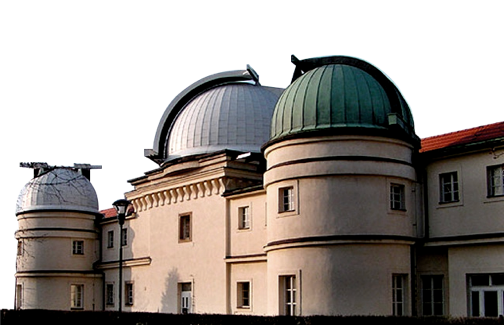
\includegraphics[width=5.9cm]{images/hp_sh.png}
\end{frame}

\section[Hackathon v Praze]{Dlouhý název sekce 1}

\subsection[Jak soutěž probíhala?]{Dlouhý název podsekce 1}
\begin{frame}{Jak soutěž probíhala?}
  \begin{columns}[T]
    \begin{column}{.6\textwidth}
    \begin{itemize}
        \item prohlídka planetária
        \item vysvětlení soutěže
        \item vymýšlení nápadů
        \item večerní umělecké promítání
        \item vytváření prezentace
        \item prezentování
        \item vyhlášení
    \end{itemize}
    \end{column}
    \begin{column}{.4\textwidth}
    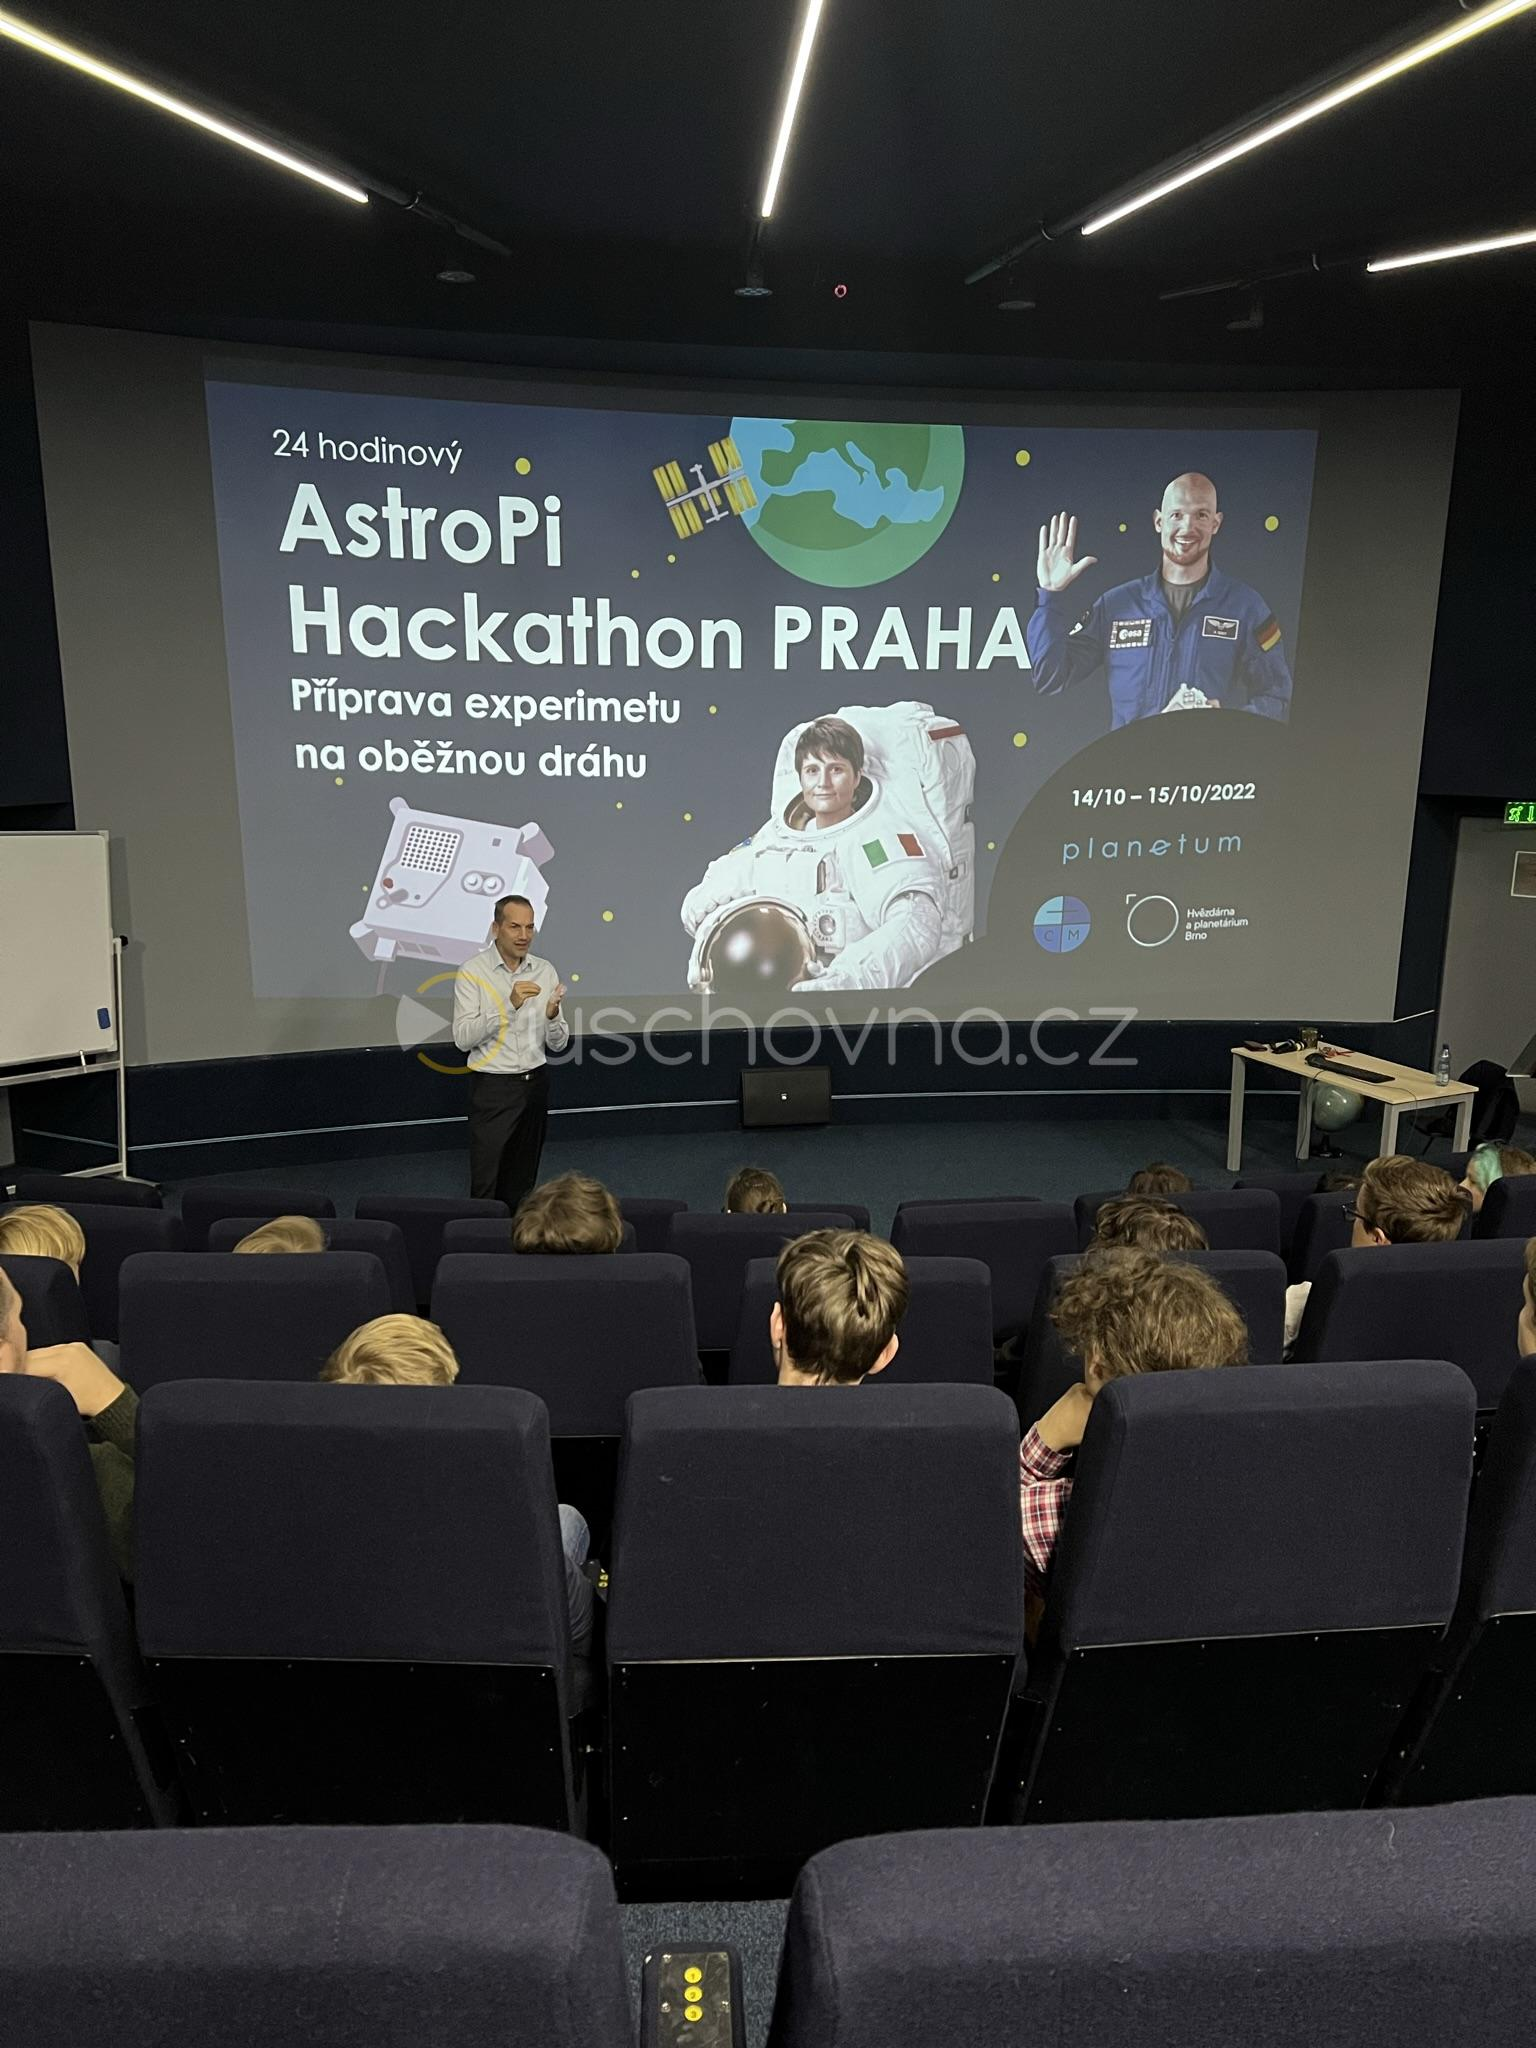
\includegraphics[width = 4cm]{images/hackathon_uvod.png}
    \end{column}
  \end{columns}
\end{frame}

\begin{frame}
\begin{figure}
  \includegraphics[height = 6.5cm,keepaspectratio]{images/fotky.png}
  \caption{Nejvíce nás potěšila chálka%
    \footnote{%c
    chálka = potrava, jídlo
    }%
  }
\end{figure}
\end{frame}

\subsection[Co jsme vymysleli?]{Dlouhý název podsekce 1}
\begin{frame}{Co jsme vymysleli?}
  \begin{columns}[T]
    \begin{column}{.6\textwidth}
    \begin{itemize}
        \item spoustu nerealizovatelných nápadů
        \begin{itemize}
            \item rozpoznání krajiny
            \item velikost měst v závislosti na světle
        \end{itemize}
        \item určování \alert{výšky mraku}
        \begin{itemize}
            \item s pomocí stínu
            \item možné určení typu mraku
        \end{itemize}
        \item nutný záložní plán
    \end{itemize}
    \end{column}
    \begin{column}{.4\textwidth}   \end{column}
  \end{columns}
  \begin{columns}[T]
        \begin{column}{.5\textwidth}
        \vspace{0.3cm}
            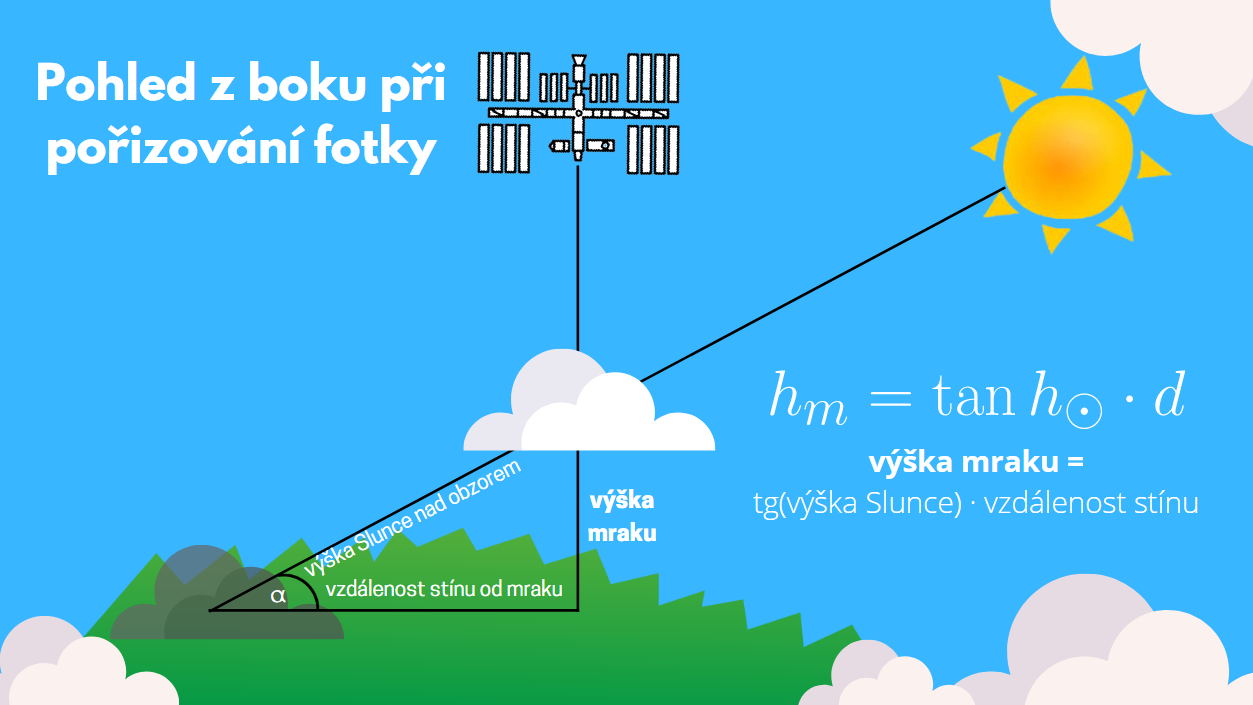
\includegraphics[width=\textwidth]{images/Prezentace-2.png}
        \end{column}
        \begin{column}{.5\textwidth}
            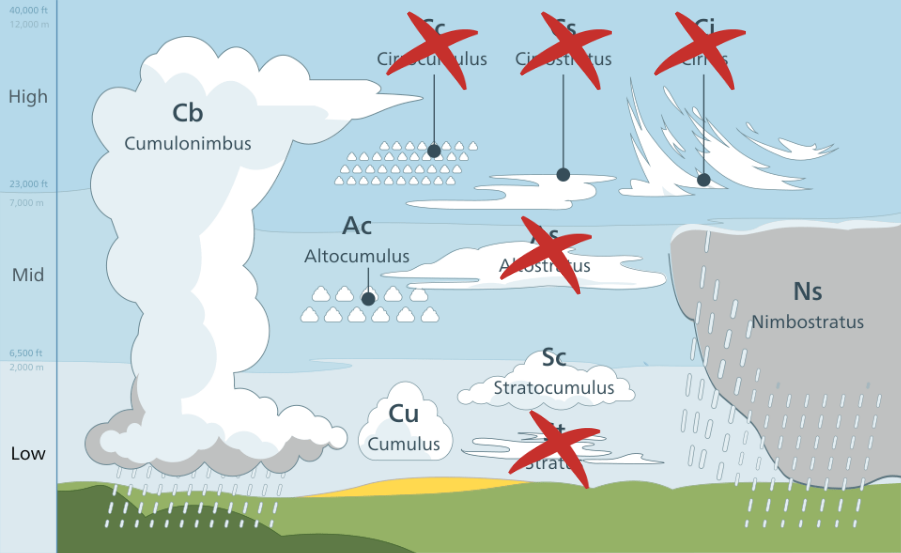
\includegraphics[width=\textwidth]{images/typy mraku.png}
        \end{column}
  \end{columns}
\end{frame}

\subsection[Co jsme vymysleli?]{Dlouhý název podsekce 1}
\begin{frame}{Prezentace nápadu v Praze}
     \begin{columns}[T]
        \begin{column}{.7\textwidth}
            \begin{itemize}
                \item prezentace před tříčlennou porotou
            \end{itemize}
        \end{column}
        \begin{column}{.3\textwidth}
        \vspace{-1.45cm}
            
\includegraphics[width=2cm]{images/qr-code.png}
        \end{column}
    \end{columns}
    
    \vspace{0.1cm}
    \begin{center}
        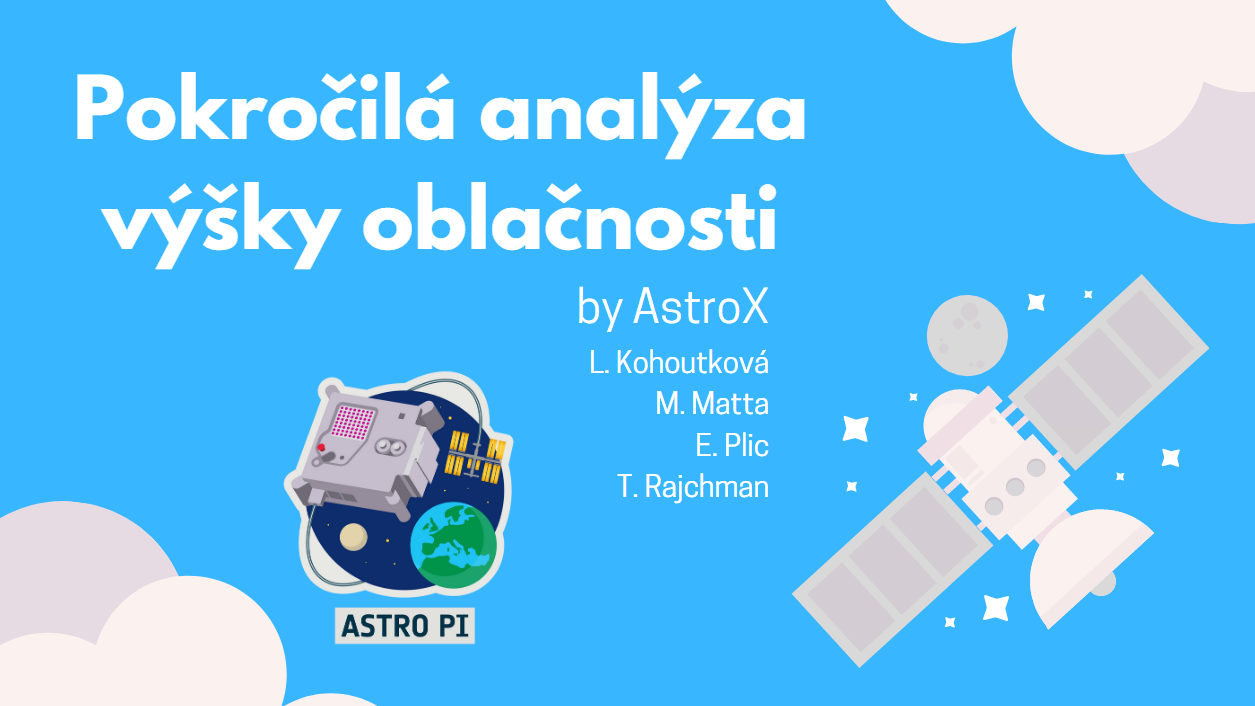
\includegraphics[width=10cm]{images/Prezentace-1.png}
    \end{center}
\end{frame}

\begin{frame}{Prezentace nápadu}
    \vspace{0.1cm}
    \begin{center}
        
\includegraphics[width=10cm]{images/Prezentace-3.png}
    \end{center}  
\end{frame}

\begin{frame}{Prezentace nápadu v Praze}
    \vspace{0cm}
    \begin{center}
        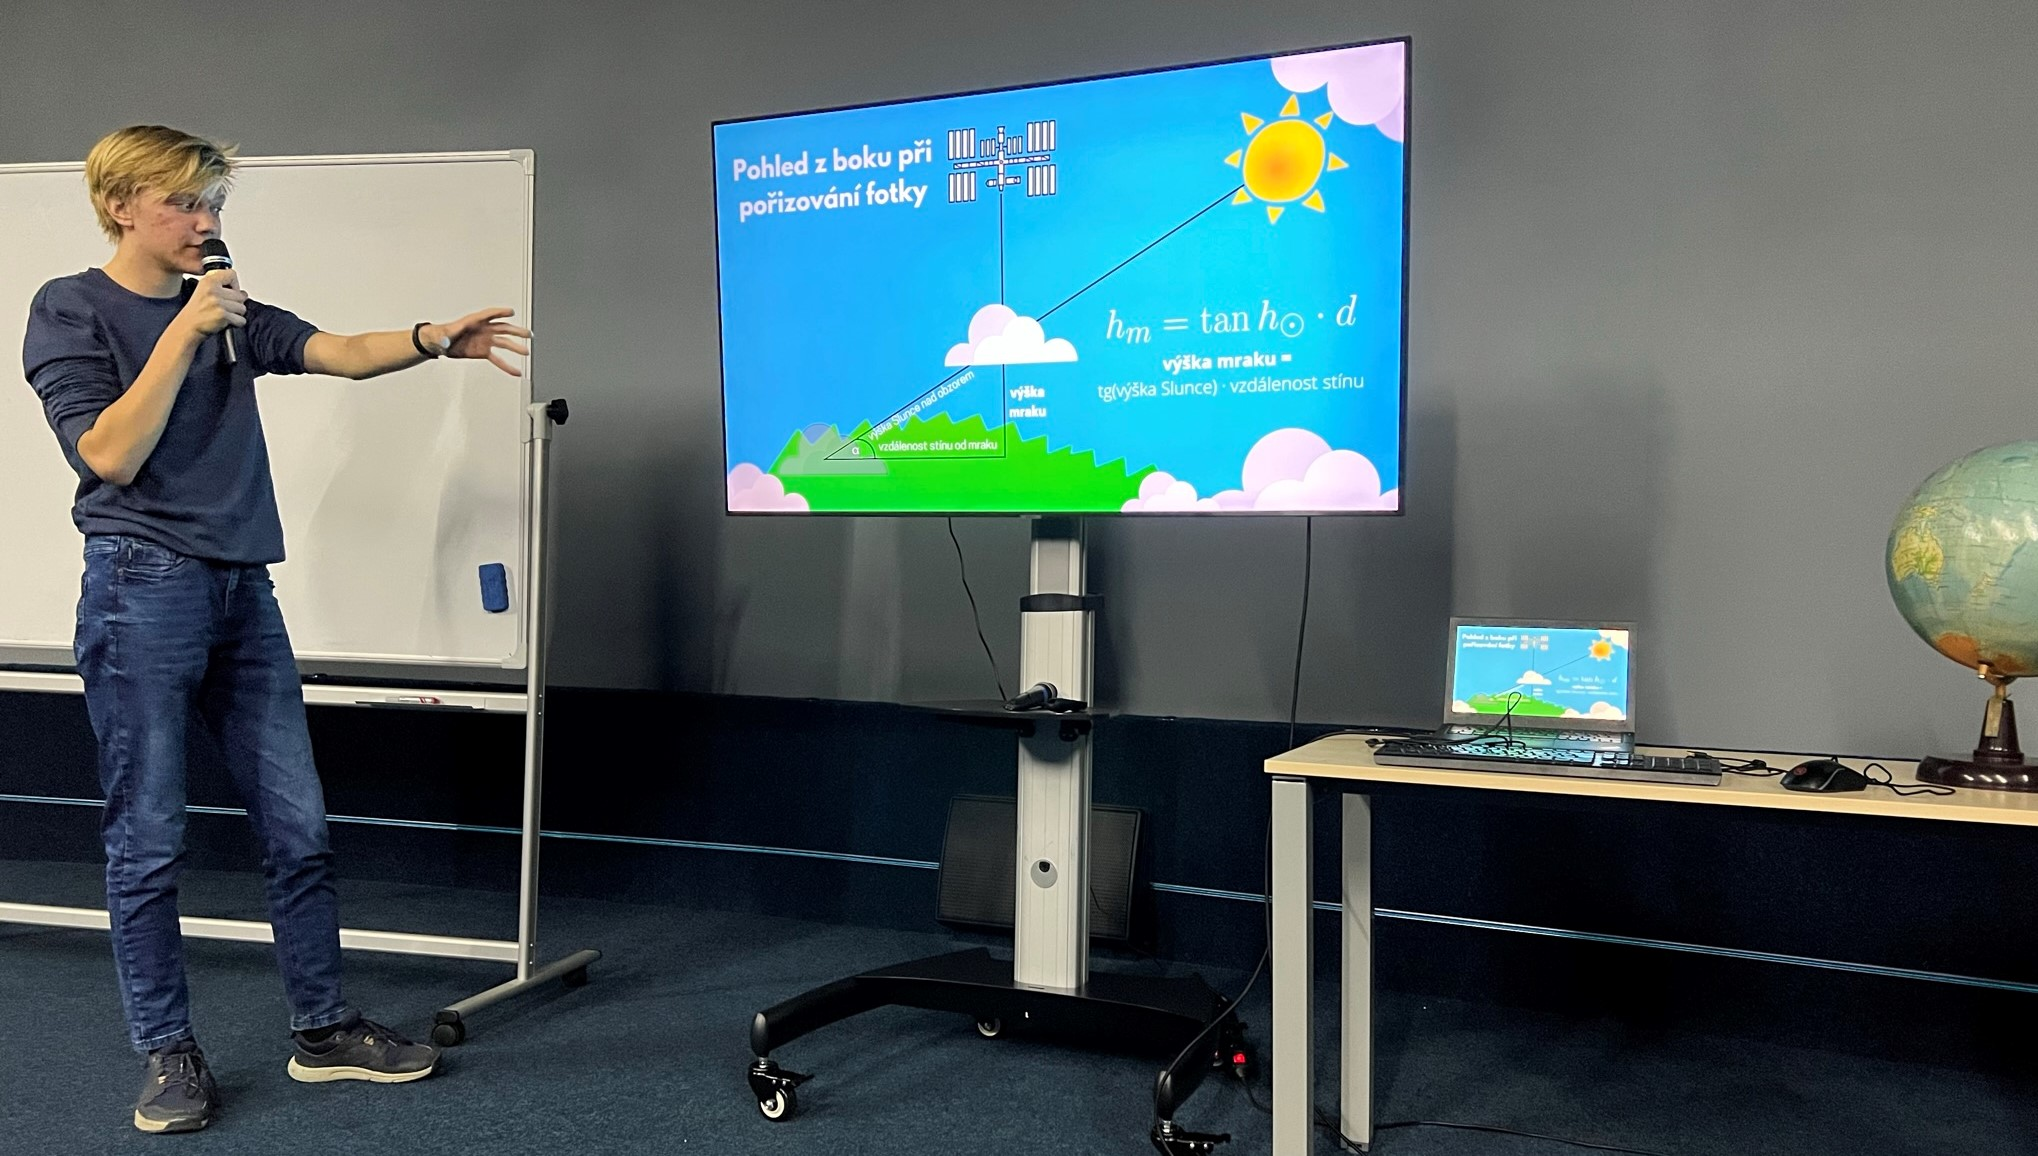
\includegraphics[width=10cm]{images/IMG_0098_2.png}
    \end{center}  
\end{frame}


\subsection[Co jsme vymysleli?]{Dlouhý název podsekce 1}
\begin{frame}{Výhra v Praze}
    \begin{itemize}
        \item z 6 týmů jsme obsadili \alert{1. místo} 
    \end{itemize}
\begin{columns}[T]
    \begin{column}{.5\textwidth}
        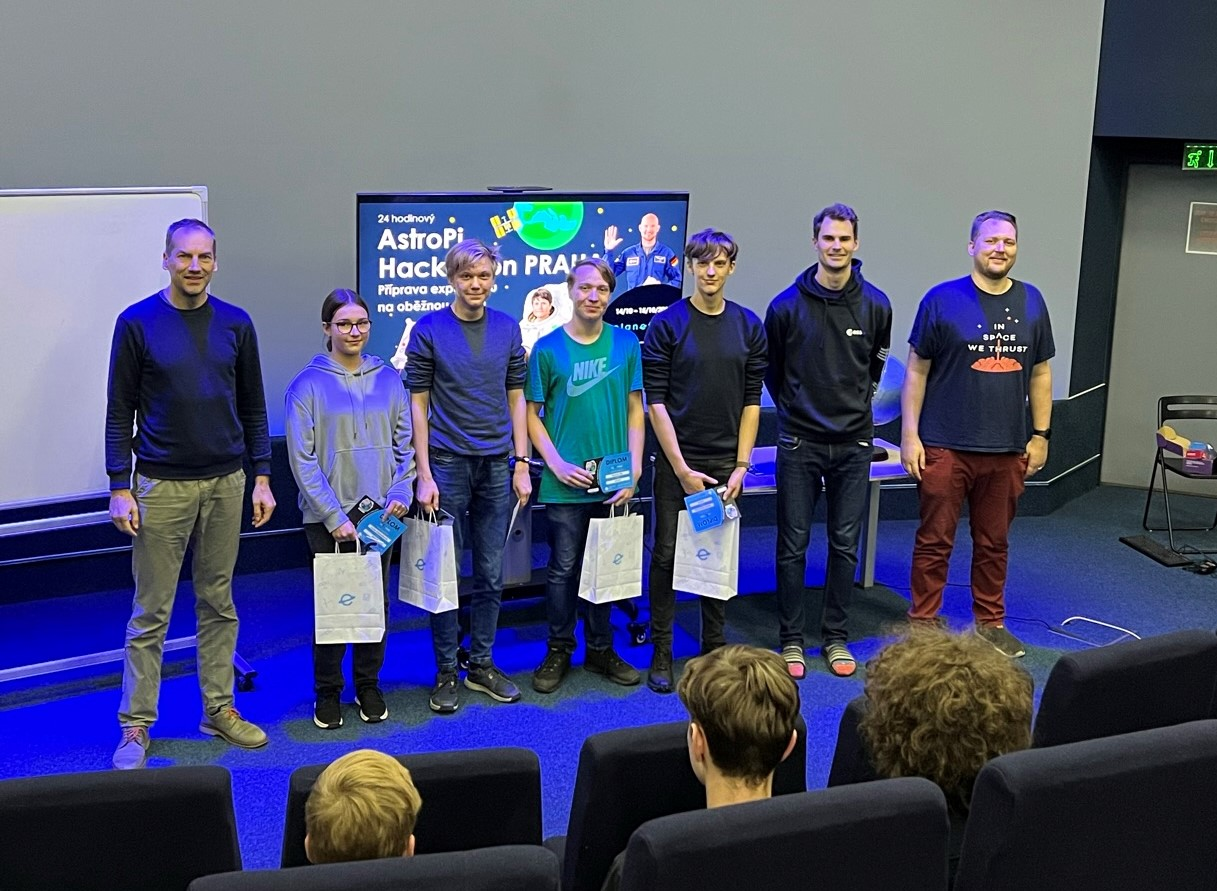
\includegraphics[width=1\textwidth]{images/vyhravsichni.jpeg}    
    \end{column}
    \begin{column}{.5\textwidth}
        \vspace{2cm}
        \hspace{0.1cm}    \includegraphics[width=1\textwidth]{images/diplom_final.png}    
    \end{column}
  
\end{columns}
\end{frame}

\section{Přihláška na fázi 2}
\subsection[Poslání návrhu]{Dlouhý název podsekce 1}
\begin{frame}{Jak jsme návrh odeslali?}
     \begin{columns}[T]
        \begin{column}{.7\textwidth}
            \begin{itemize}
                \item museli jsme připravit text a odpovědět na zadané otázky
            \end{itemize}
        \end{column}
        \begin{column}{.3\textwidth}
        \end{column}
    \end{columns}

    \vspace{4.1cm}
    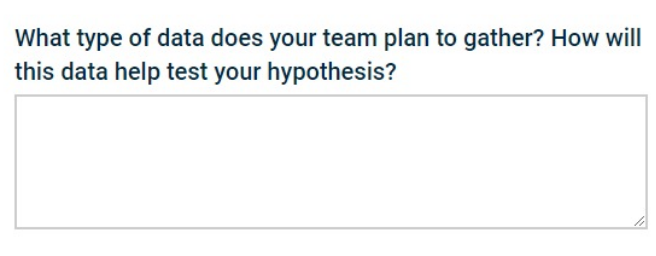
\includegraphics[height=2cm]{images/esa_otazky_1.png}
    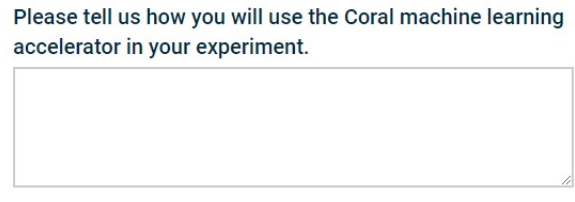
\includegraphics[height=2cm]{images/esa_otazky_2.png}
\end{frame}

\begin{frame}{Odpověď}
\begin{itemize}
                    \item náš návrh byl v prosinci \alert{schválen}
\end{itemize}
\begin{center}
    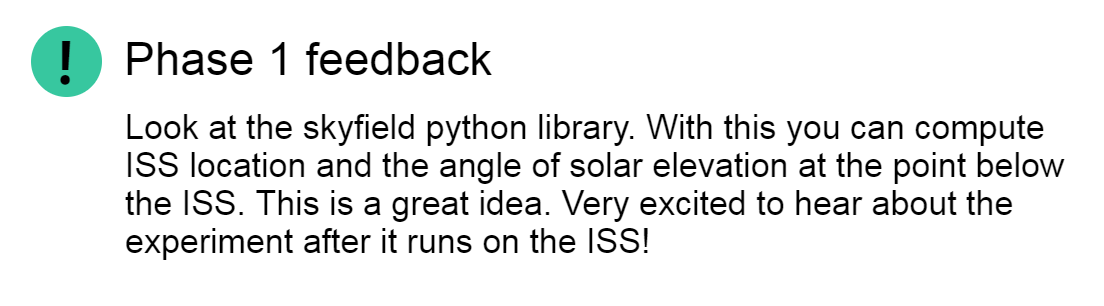
\includegraphics[width=10cm]{images/feedback.png}
   
\end{center}
\end{frame}

\begin{frame}{Obdržení sady}
\begin{columns}[T]
        \begin{column}{.5\textwidth}
\begin{itemize}
                    \item poté jsme obdrželi sadu \alert{Raspberry Pi} s příslušenstvím až z \alert{Nizozemska}
\end{itemize}
\vspace{1cm}
    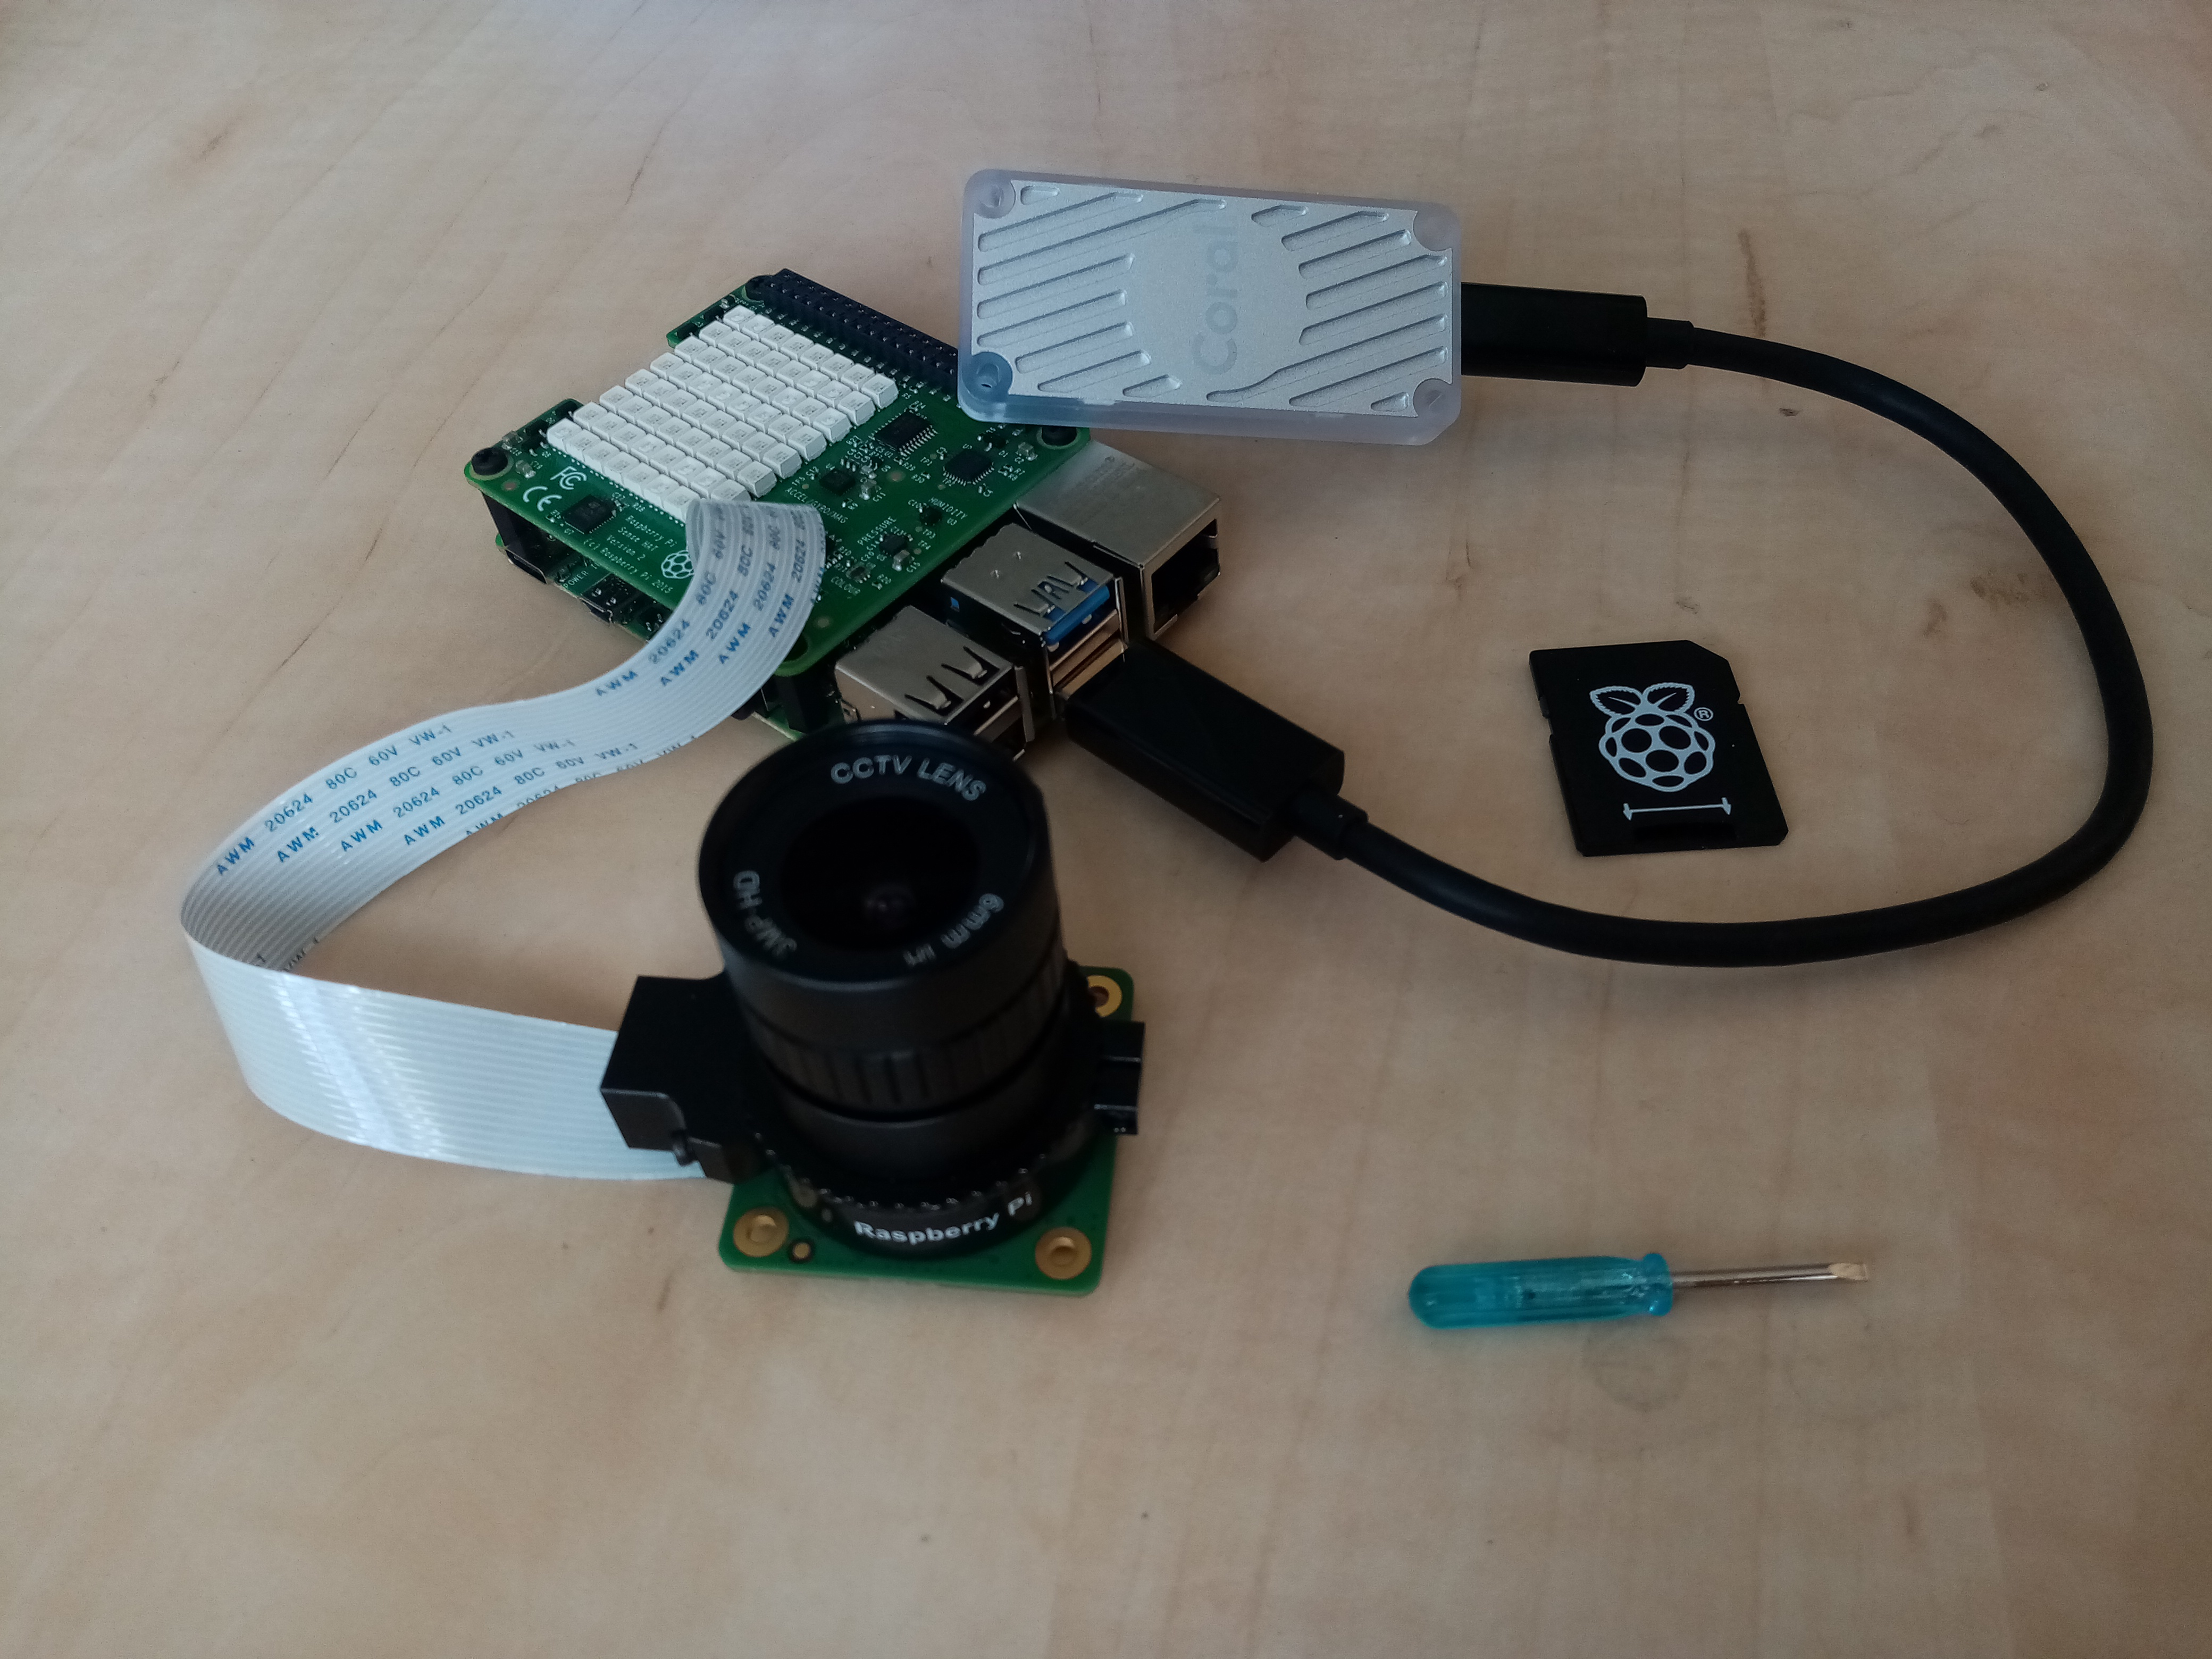
\includegraphics[width=\textwidth]{images/rozbalenasada.jpg}

        \end{column}
        \begin{column}{.5\textwidth}
        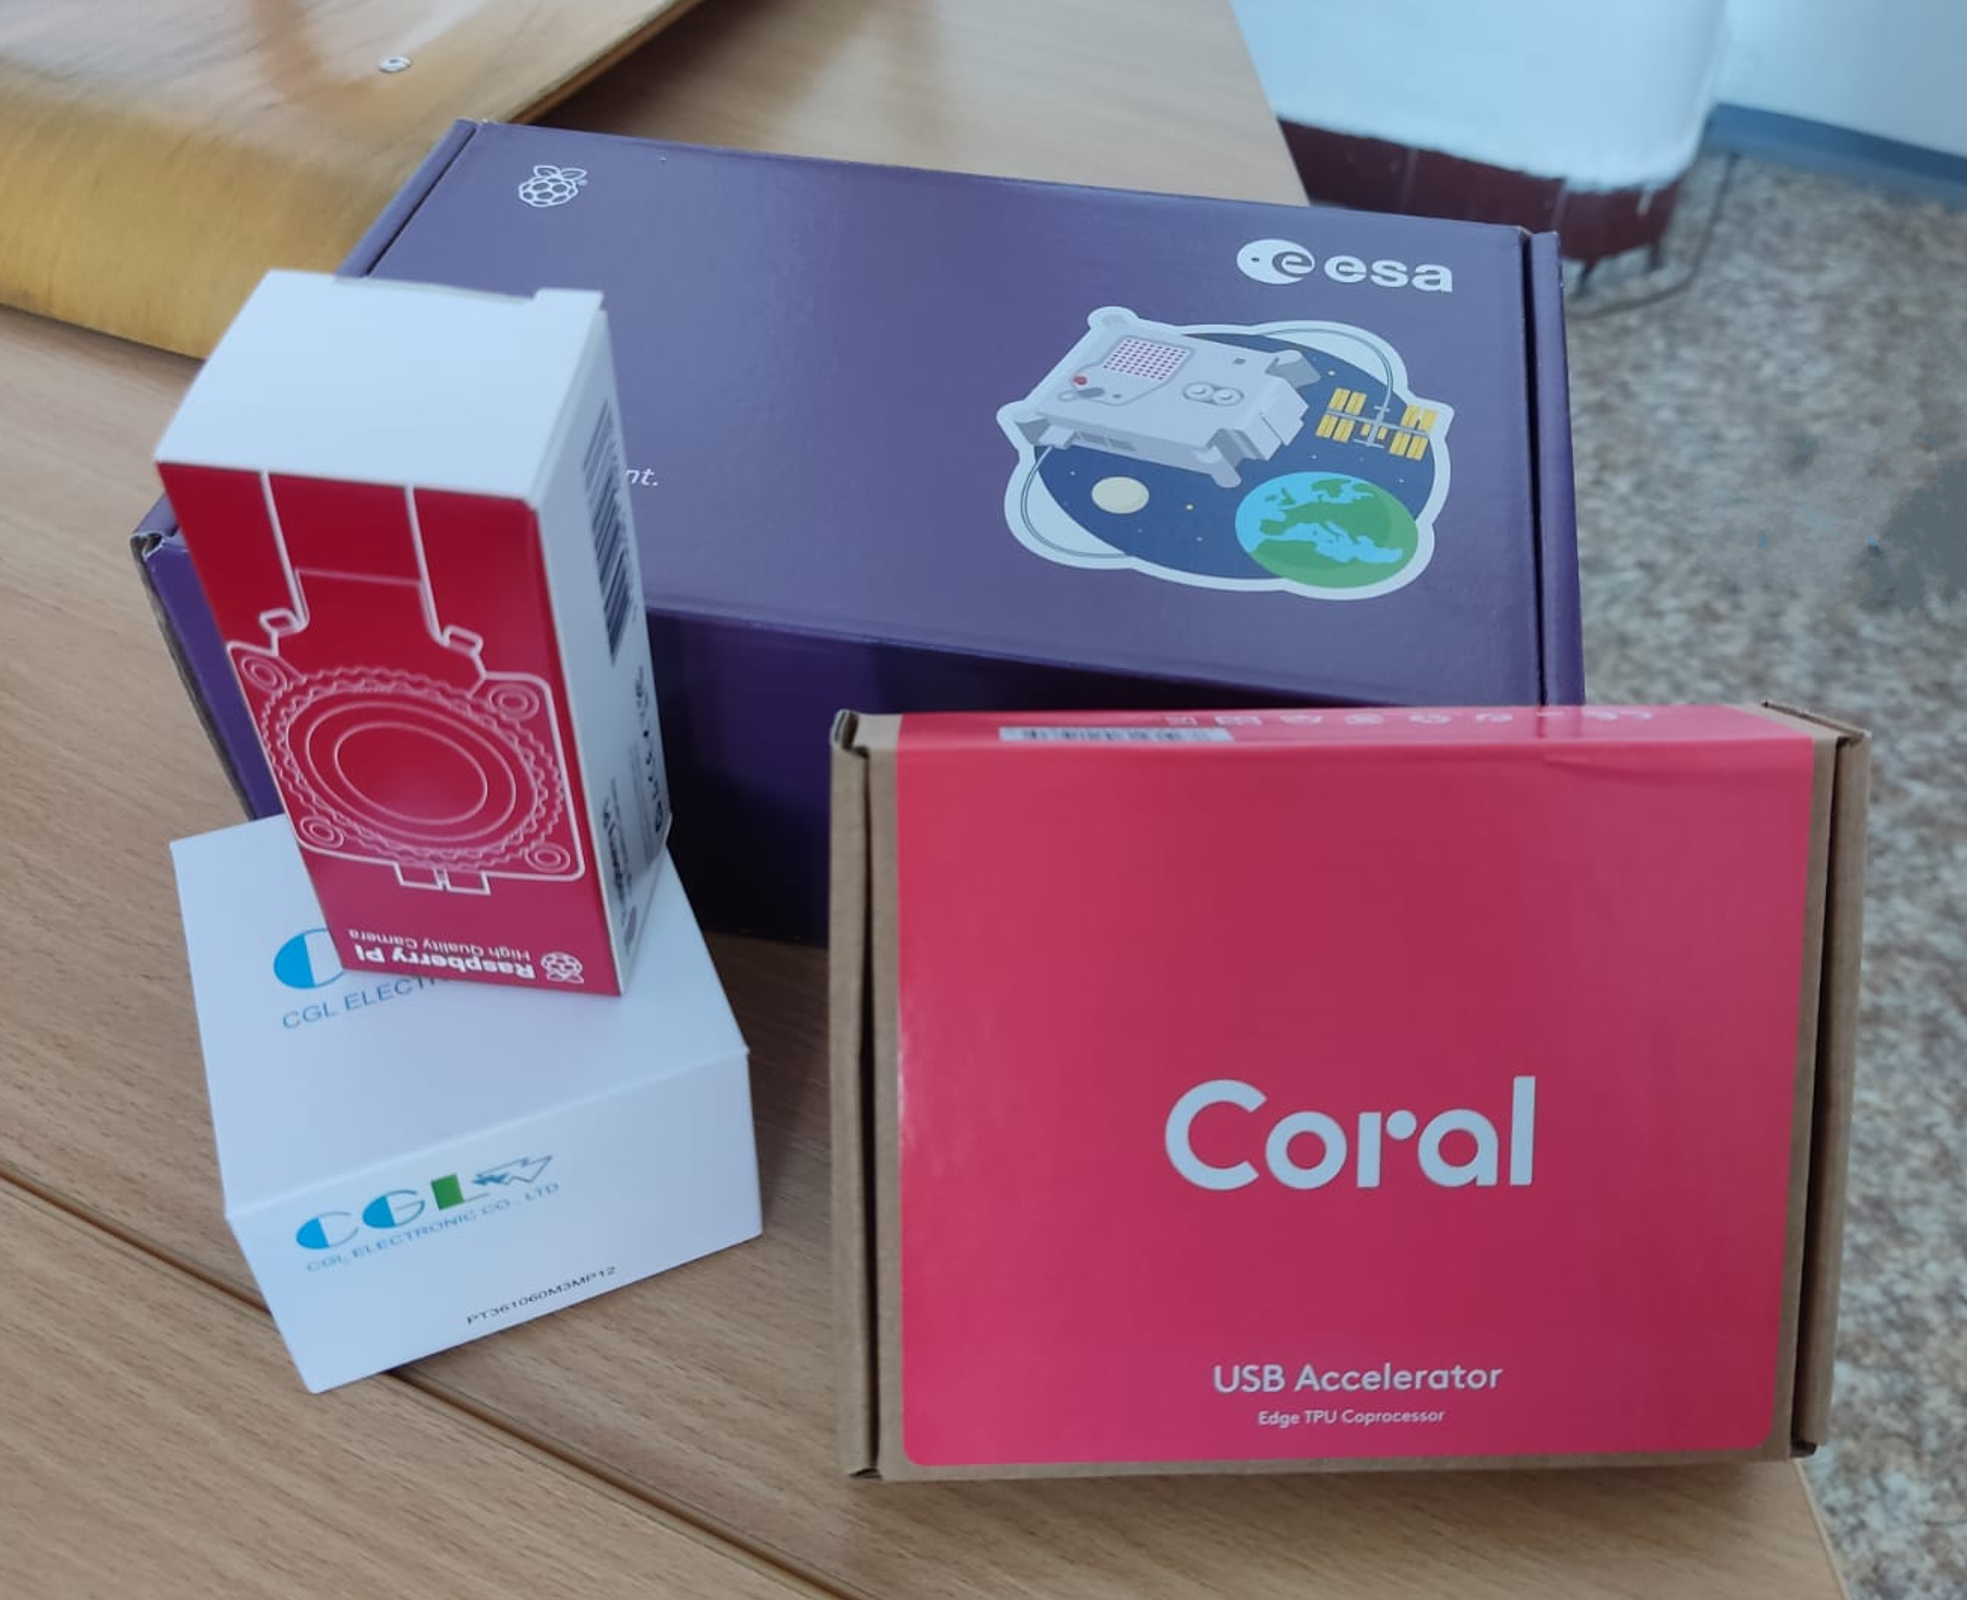
\includegraphics[width=\textwidth]{images/baleni.png}
        \end{column}
\end{columns}
\end{frame}

\begin{frame}{Senzory AstroPi počítače}
    \begin{columns}[T]
            \begin{column}{.5\textwidth}
                \begin{itemize}
                    \item PIR senzor (passive infrared, senzor pohybu)
                    \item senzor barvy a svítivosti
                    \item gyroskop, akcelometr, magnetometr
                    \item senzor teploty
                    \item senzor vzdušné vlhkosti
                    \item senzor tlaku
                    \item kamera
                \end{itemize}
                \vspace{1cm}
            \end{column}
            \begin{column}{.5\textwidth}
            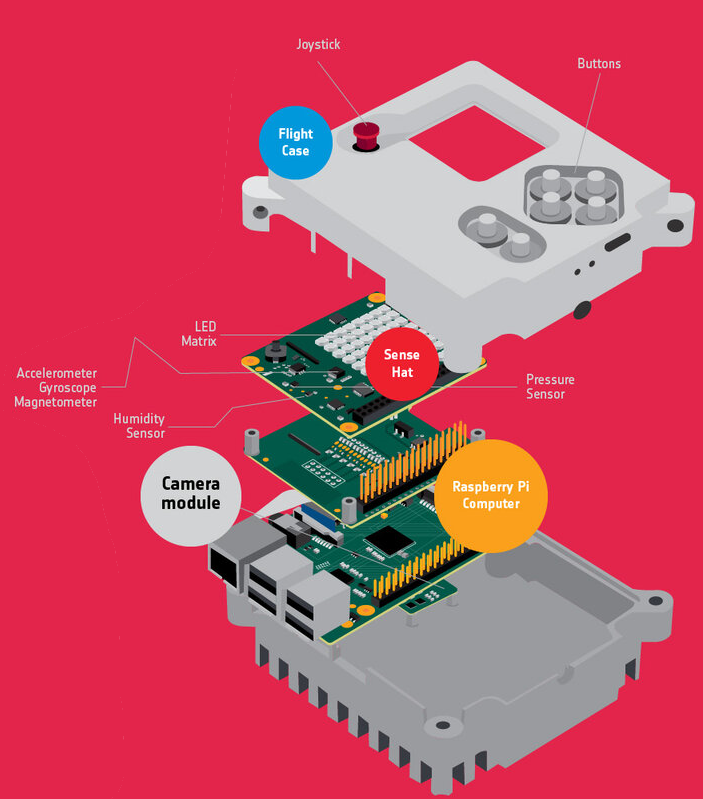
\includegraphics[width=\textwidth]{images/senzory_raspberry.png}
            \end{column}
    \end{columns}
\end{frame}

\section{Práce na FAV}
\subsection[Proč jsme potřebovali být na FAV?]{Dlouhý název podsekce 1}
\begin{frame}{Proč jsme potřebovali být na FAV?}
     \begin{columns}[T]
        \begin{column}{.7\textwidth}
            \begin{itemize}
                \item ve škole nebylo možné žádnou učebnu vyblokovat na 8 hodin
                \item školní \alert{internet} (studenti MG ví)
                \item těžká koordinace projektu z domova
            \end{itemize}
        \end{column}
        \begin{column}{.3\textwidth}
        \end{column}
    \end{columns}
\end{frame}

\subsection[Jak jsme se na FAV dostali?]{Dlouhý název podsekce 1}
\begin{frame}{Jak jsme se na FAV dostali?}
     \begin{columns}[T]
        \begin{column}{.7\textwidth}
            \begin{itemize}
                \item napsali jsme email doporučenému kontaktu podle stránek ZČU
                \item dostali jsme odpověď od doc. Vášy
                \item nápad jsme představili doc. Vášovi a doc. Masopustovi
                \item domluvili jsme se a dostali jsme \alert{laboratoř} s vybavením
            \end{itemize}
        \end{column}
        \begin{column}{.3\textwidth}
        \end{column}
    \end{columns}
\end{frame}

\subsection[Laboratoř na FAV]{Dlouhý název podsekce 1}
\begin{frame}[c]
    \begin{center}
    \color{mubeamer@base}
    \huge{\textbf{Laboratoř na FAV}}
    \vspace{1mm}

    \Large UC 355 - “Holodíra”
    \end{center}
\end{frame}

\begin{frame}[plain]
    \fullsizegraphic{images/laborka_1.jpg}
\end{frame}

\begin{frame}[plain]
    \fullsizegraphic{images/laborka_2.jpg}    
\end{frame}

\begin{frame}[plain]
    \fullsizegraphic{images/laborka_3.jpg}    
\end{frame}

\begin{frame}[plain]
    \fullsizegraphic{images/laborka_4.jpg}    
\end{frame}

\section{Program}
\subsection[class \texttt{ai}]{Dlouhý název podsekce 1}

\begin{frame}[c]
\begin{center}
\color{mubeamer@base}
\Huge \textbf{Jak detekovat mraky?}
\end{center}
\end{frame}

\begin{frame}{Použít RS-Net\footnote{Remote Sensing Network} deep learning}
     \begin{columns}[T]
        \begin{column}{.45\textwidth}
            \begin{itemize}
                \item po přečtení několika studií o RS-Net \cite{jeppesen2019cloud} architektuře jsme mysleli, že by se tento kód dal použít
                \item metoda postupně se zmenšujících bounding boxů
            \footnotemark 
                \item pro komplikovanost jsme nebyli schopni tuto metodu aplikovat
            \end{itemize}
        \end{column}
        \begin{column}{.45\textwidth}
            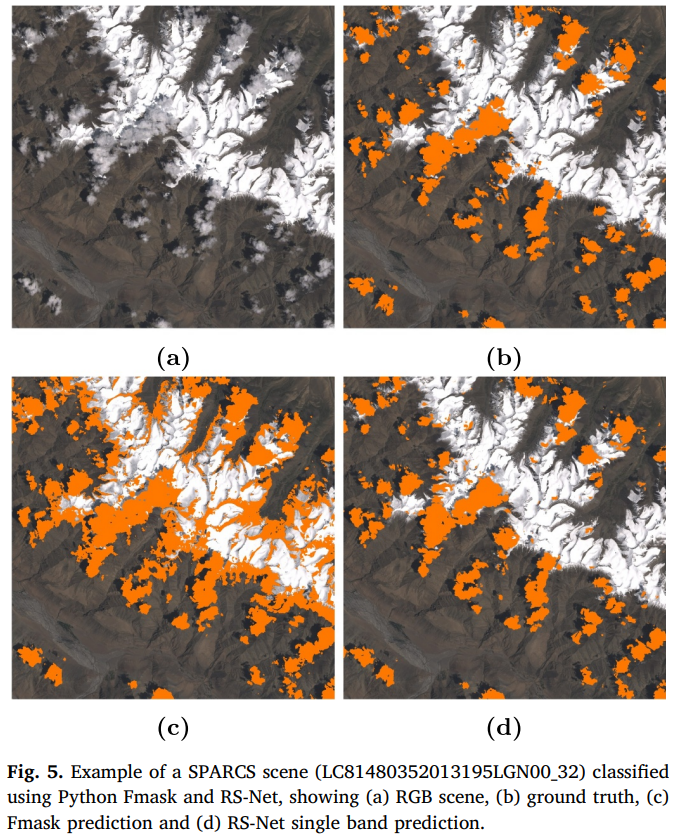
\includegraphics[width=1\textwidth]{images/rs-net.png}
        \end{column}
    \end{columns}
    \footnotetext{čtveřice souřadnic ohraničující objekt, reprezentován čtvercem}
\end{frame}

\begin{frame}{Bounding box umělá inteligence}
     \begin{columns}[T]
        \begin{column}{.45\textwidth}
            \begin{itemize}
                \item mohli jsme vytrénovat jednoduchý model na detekci mraků a stínů
                \item poté by stačilo udělat jednoduchý výpočet a zjistili bychom výšku
                \item detekce stínů se ukázala být příliš komplikovaná a nespolehlivá
                \item detekce mraků touto metodou se však ukázala být nejjednodušším řešením, takže jsme s ní dále pracovali
            \end{itemize}
        \end{column}
        \begin{column}{.45\textwidth}
            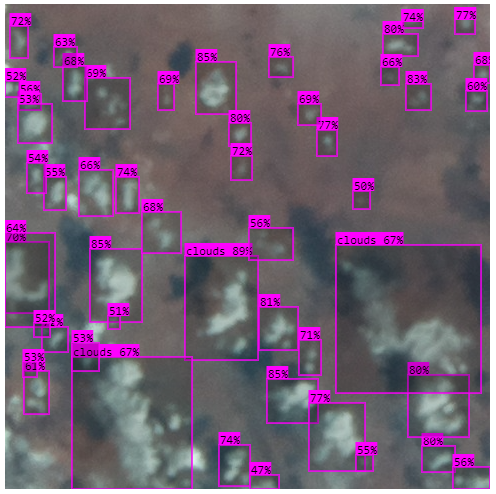
\includegraphics[width=1\textwidth]{images/model_test.png}
        \end{column}
    \end{columns}
\end{frame}

\begin{frame}[c]
\begin{center}
\color{mubeamer@base}
\Huge \textbf{Jak se trénuje\\ „umělá inteligence“?}
\end{center}
\end{frame}

\begin{frame}{Co je to umělá inteligence?}
     \begin{columns}[T]
        \begin{column}{.8\textwidth}
            \begin{itemize}
                \item poslední dobou spíše catchword\footnotemark 
                \item přesnějším popisem našeho využití je \alert{strojové učení}
                \item modelu je předložen dataset\footnotemark  obsahující velké množství informací
                \item model v datech postupně začne hledat spojitosti a závislosti
                \item při dostatečném množství trénovacích dat je pak model schopen nalézt výsledky i na obrázcích, které neobsahují anotace\footnotemark[6]
            \end{itemize}
        \end{column}
        \begin{column}{.2\textwidth}
            
\includegraphics[width=0.7\textwidth]{images/Tensorflow_logo.svg.png}
        \end{column}
    \end{columns}
    \footnotetext[4]{slovo, které vyvolává speciální pozornost}
    \footnotetext[5]{soubor obrázků obsahující anotované\footnotemark[6] objekty}
    \footnotetext[6]{soubory souřadnic ohraničující objekty}
\end{frame}

\begin{frame}{Jak se připravuje dataset?}
     \begin{columns}[T]
        \begin{column}{.8\textwidth}
            \begin{itemize}
                \item použili jsme \alert{Roboflow}\footnotemark[7] 
                \item sehnali jsme obrázky z minulého ročníku Astro Pi
                \item vybrali jsme 16 obrázků (pozor na overfitting\footnotemark[8])
                \item rozřezali jsme je na 16 sektorů
                \item ručně jsme udělali bounding box anotace
            \end{itemize}
        \end{column}
        \begin{column}{.2\textwidth}
            \vspace{4cm}
            
\includegraphics[width=1\textwidth]{images/roboflow.jpg}
        \end{column}
    \end{columns}
    \footnotetext[7]{online služba umožňující kolaboraci na anotaci společného datasetu}
    \footnotetext[8]{trénování modelu na příliš ideálních datech}
\end{frame}

\begin{frame}[plain]
\fullsizegraphic{images/crop_example.png}
\end{frame}

\begin{frame}{Jak jsme získali model?}
     \begin{columns}[T]
        \begin{column}{.9\textwidth}
            \begin{itemize}
                \item použili jsme Jupyter \href{http://tiny.cc/tutorialtflite}{notebook}\footnotemark[9] podle YouTube videa \cite{tflitetutorial} 
                \item vytrénovali jsme Tensorflow\footnotemark[10] 1.x model a překonvertovali jsme jej na kvantovaný \alert{TFLite} model pro Coral\footnotemark[11]
                \item použili jsme Google Colab\footnotemark[12] kvůli velkému výkonu
                \item exportovali jsme Roboflow data do .tfrecord a .xml souborů
                \item manuálně jsme vytvořili labelmap
                \item model jsme trénovali několik hodin
            \end{itemize}
        \end{column}
        \begin{column}{.1\textwidth}
        \end{column}
    \end{columns}
    \footnotetext[9]{typ souboru kombinující snipetty Python kódu a textů k instrukcím}
    \footnotetext[10]{bezplatná knihovna a platforma pro trénování modelů od Googlu}
    \footnotetext[11]{nám poskytnuté příslušenství k Raspberry Pi pro zrychlení běhu AI modelů}
    \footnotetext[12]{služba poskytující bezplatný hosting Jupyter notebooků}
\end{frame}

\begin{frame}[c]
\begin{center}
\color{mubeamer@base}
\huge{\textbf{Jak jsme model implementovali?}}
\vspace{5mm}
\Large Praktická ukázka kódu třídy \texttt{ai}
\end{center}
\end{frame}


\subsection[class \texttt{shadow}]{Dlouhý název podsekce 1}
\begin{frame}[c]
\begin{center}
\color{mubeamer@base}
\Huge \textbf{Jak detekovat stíny?}
\end{center}
\end{frame}

\begin{frame}{Cloud-shadow fingerprint}
     \begin{columns}[T]
        \begin{column}{.45\textwidth}
            \begin{itemize}
                \item svítivost jednotlivých pixelů ve směru, kde by se měl nacházet stín
                \item bod s nejvyšší svítivostí by byl mrak a bod s nejnižší svítivostí by byl stín
            \end{itemize}
            \vspace{5mm}
            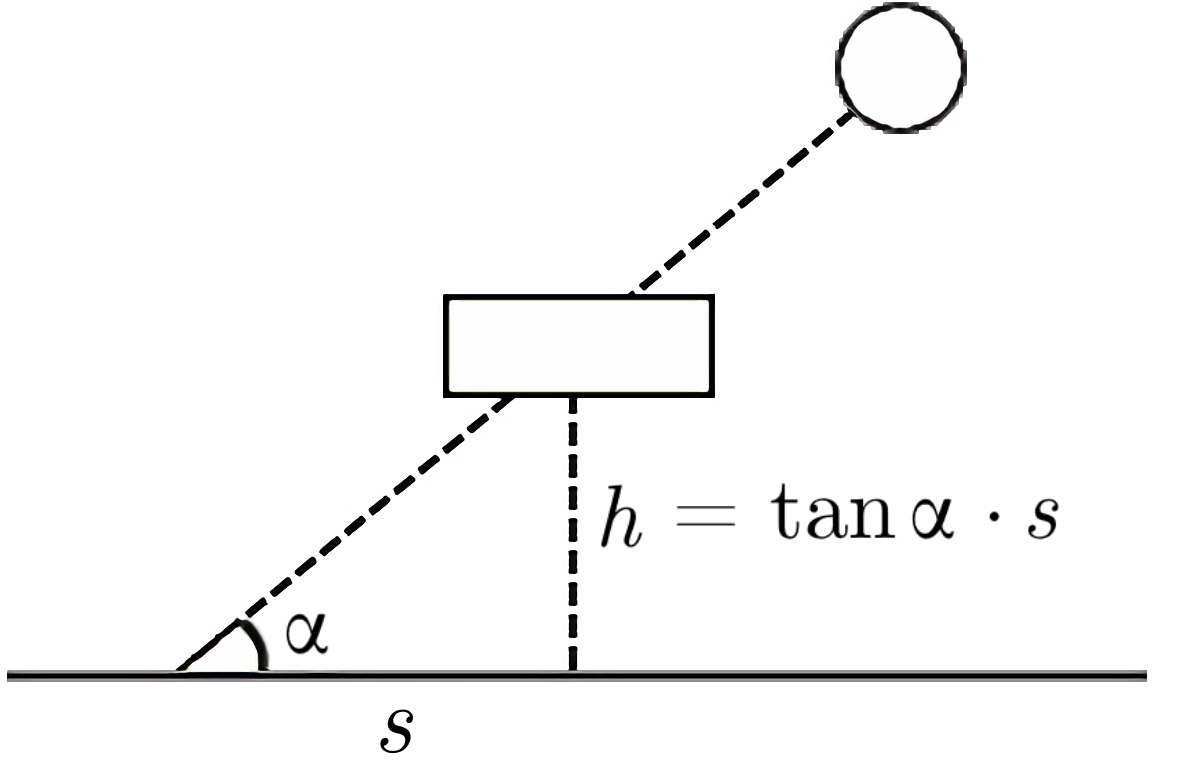
\includegraphics[width = 5.3cm]{images/angle4.png}
        \end{column}
        \begin{column}{.45\textwidth}
            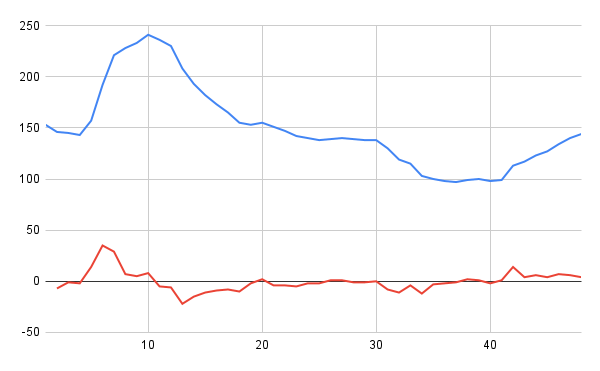
\includegraphics[width=1\textwidth]{images/chart (34).png}
            \vspace{5mm}
            \hspace{1.45cm} 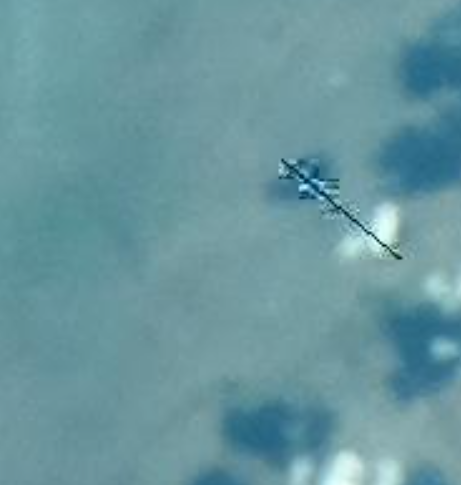
\includegraphics[width=0.7\textwidth]{images/shadow_search.png}
        \end{column}
    \end{columns}
    \begin{center}
            
    \end{center}
\end{frame}

\begin{frame}{Jakým směrem hledat stíny?}
     \begin{columns}[T]
        \begin{column}{.7\textwidth}
            \begin{itemize}
                \item stíny budou padat podle azimutu Slunce nad obzorem
                \item azimut Slunce je závislý na tom, kde je sever
                \item sever \alert{není} fixní a nedá se z fotky určit
                \item Raspberry sice má magnetometr, ale pro kvalitní určení toho, kde je stín, by se odchylky musely pohybovat v jednotkách stupňů
                \item ...alespoň to tvrdila ESA
            \end{itemize}
        \end{column}
        \begin{column}{.3\textwidth}
        \end{column}
    \end{columns}
    \begin{center}
    \end{center}
\end{frame}

\subsection[class \texttt{north}]{Dlouhý název podsekce 1}
\begin{frame}[c]
\begin{center}
\color{mubeamer@base}
\Huge \textbf{Jak zjistit sever?}
\end{center}
\end{frame}

\begin{frame}{Proč ne kompas?}
    \begin{itemize}
        \item nepřesnost \alert{20°} a nesmyslné hodnoty
    \end{itemize}
        \begin{center}
    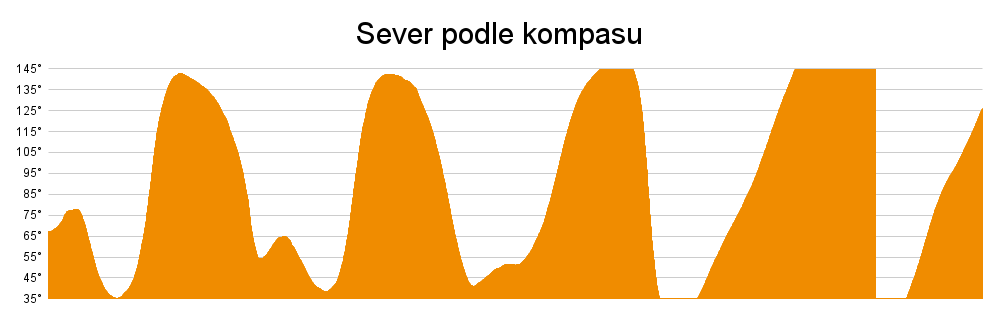
\includegraphics[height=0.4\textheight]{images/SeverPodleKompasu.png}
    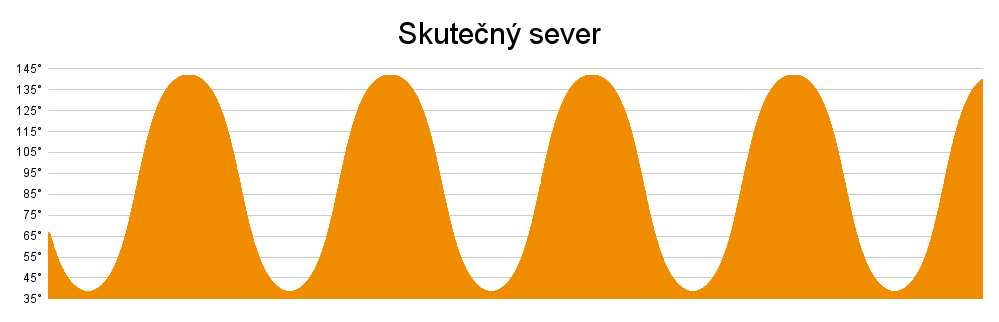
\includegraphics[height=0.4\textheight]{images/SkutecnySever.png}
    \end{center}
\end{frame}

\begin{frame}{Sever vůči ISS}
    \begin{itemize}
        \item dá zjistit pomocí sférického trojúhelníku
    \end{itemize}
    \begin{center}
        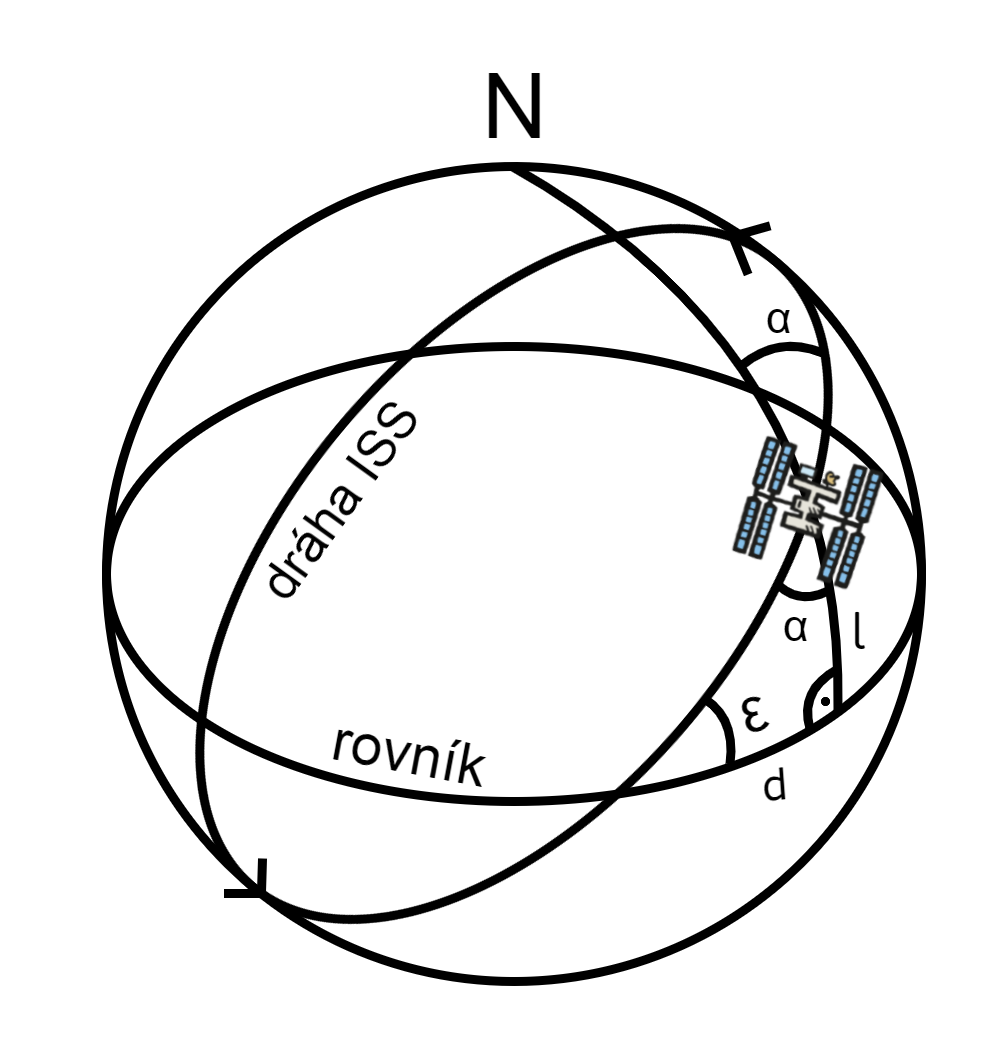
\includegraphics[width=0.4\textwidth]{images/ISS.png}\\    
    \end{center}
, kde $\alpha$ je úhel mezi severem a směrem pohybu ISS, $\varepsilon$ je sklon dráhy ISS vzhledem k rovníku, $l$ je zeměpisná šířka a $d$ je pomocná proměnná, něco jako zeměpisná délka
\end{frame}

\begin{frame}{Sever vůči ISS}
     \begin{columns}[T]
        \begin{column}{.8\textwidth}
            \begin{itemize}
                \item použijeme \alert{sférickou sinová větu}
                $$\frac{\sin(d)}{\sin(\alpha)}=\frac{\sin(l)}{\sin(\varepsilon)}~\Rightarrow\sin(d)=\frac{\sin(l)}{\sin(\varepsilon)}\sin(\alpha)~$$
                \item \alert{kotangentový vzorec} pro čtyři parametry:
                $$\cos(90\degree)\cos(d)=\cot(l)\sin(d)-\cot(\varepsilon)\sin(90\degree)$$
                $$\cot(\varepsilon)=\cot(l)\sin(d)$$
                \item zkombinujeme
                $$\cot(\varepsilon)=\cot(l)\frac{\sin(l)}{\sin(\varepsilon)}\sin(\alpha)~\Rightarrow~\sin(\alpha)=\frac{\cos(\varepsilon)}{\cos(l)}$$
            \end{itemize}
        \end{column}
        \begin{column}{.2\textwidth}
            \begin{center}
                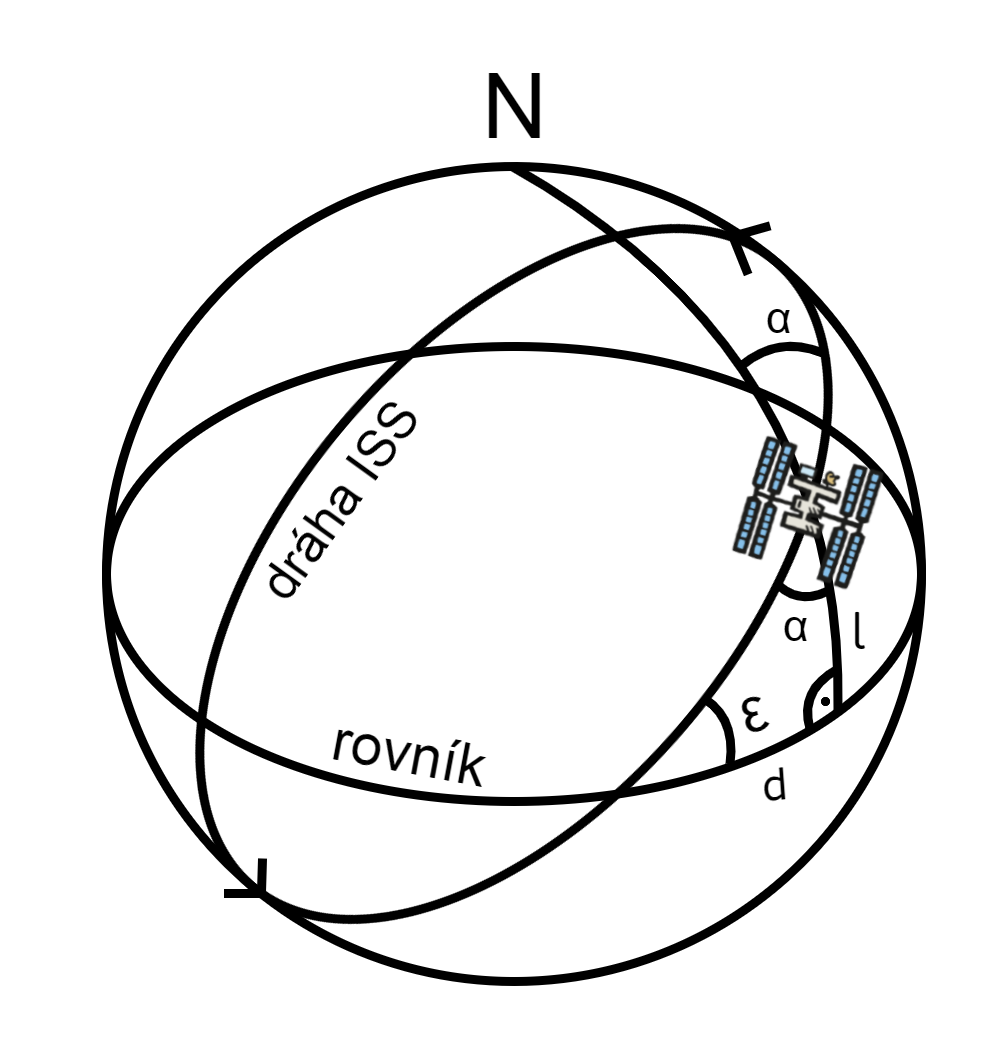
\includegraphics[width=1\textwidth]{images/ISS.png}    
            \end{center}
        \end{column}
    \end{columns}
\end{frame}

\begin{frame}{Quo vadis ISS}
     \begin{columns}[T]
        \begin{column}{.8\textwidth}
            \begin{itemize}
                \item konečná závislost $\alpha$ na zeměpisné šířce
                $$\alpha=\arcsin\left(\frac{\cos(\varepsilon)}{\cos(l)}\right)$$
                \item vzorec vrátí ostrý úhel $\rightarrow$ nutná korekce $\alpha$:
                \begin{itemize}
                    \item \alert{stoupající} šířka - úhel \alert{zůstává}
                    \item \alert{klesající} šířka - vezme se jeho \alert{doplněk ke 180\degree}
                \end{itemize}
            \end{itemize}
        \end{column}
        \begin{column}{.2\textwidth}
            \begin{center}
                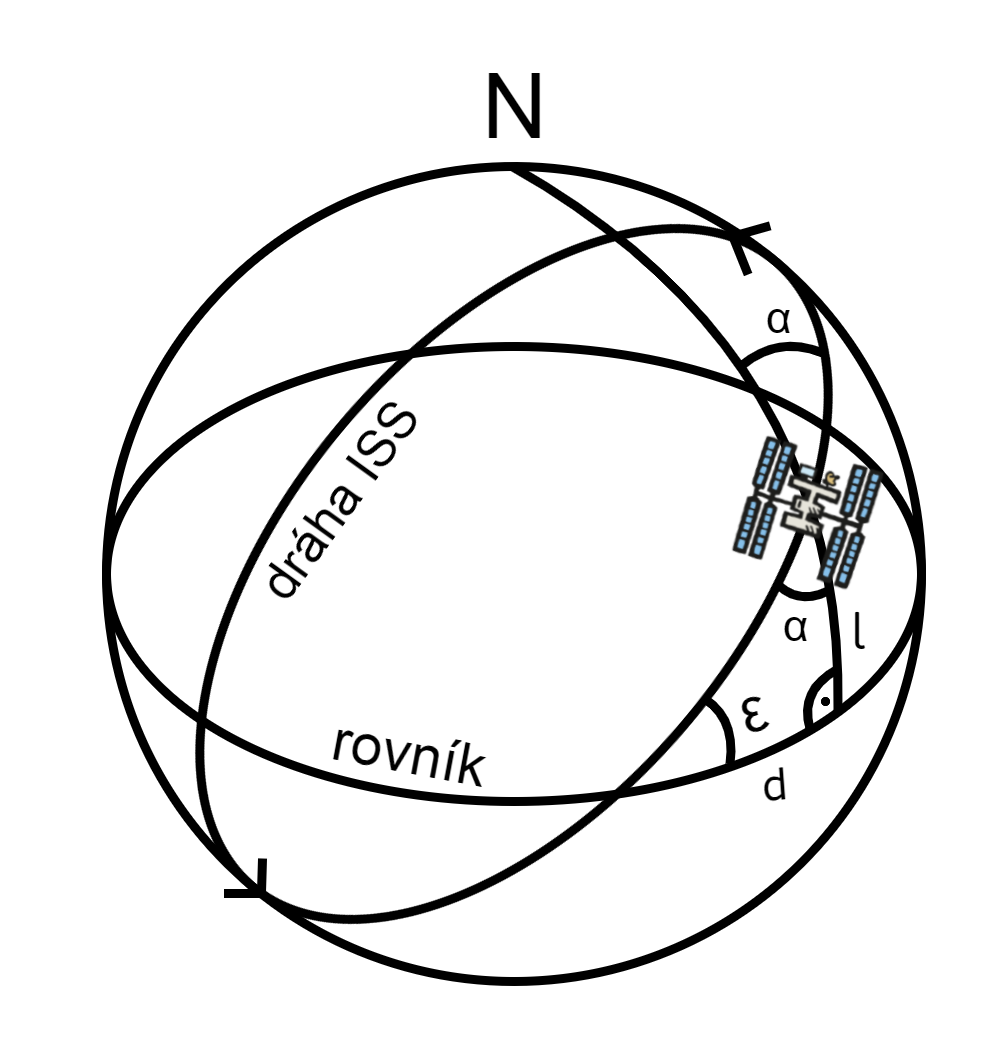
\includegraphics[width=1\textwidth]{images/ISS.png}  
            \end{center}
        \end{column}
    \end{columns}
\end{frame}
\begin{frame}{Sever vůči ISS}
            \begin{center}
            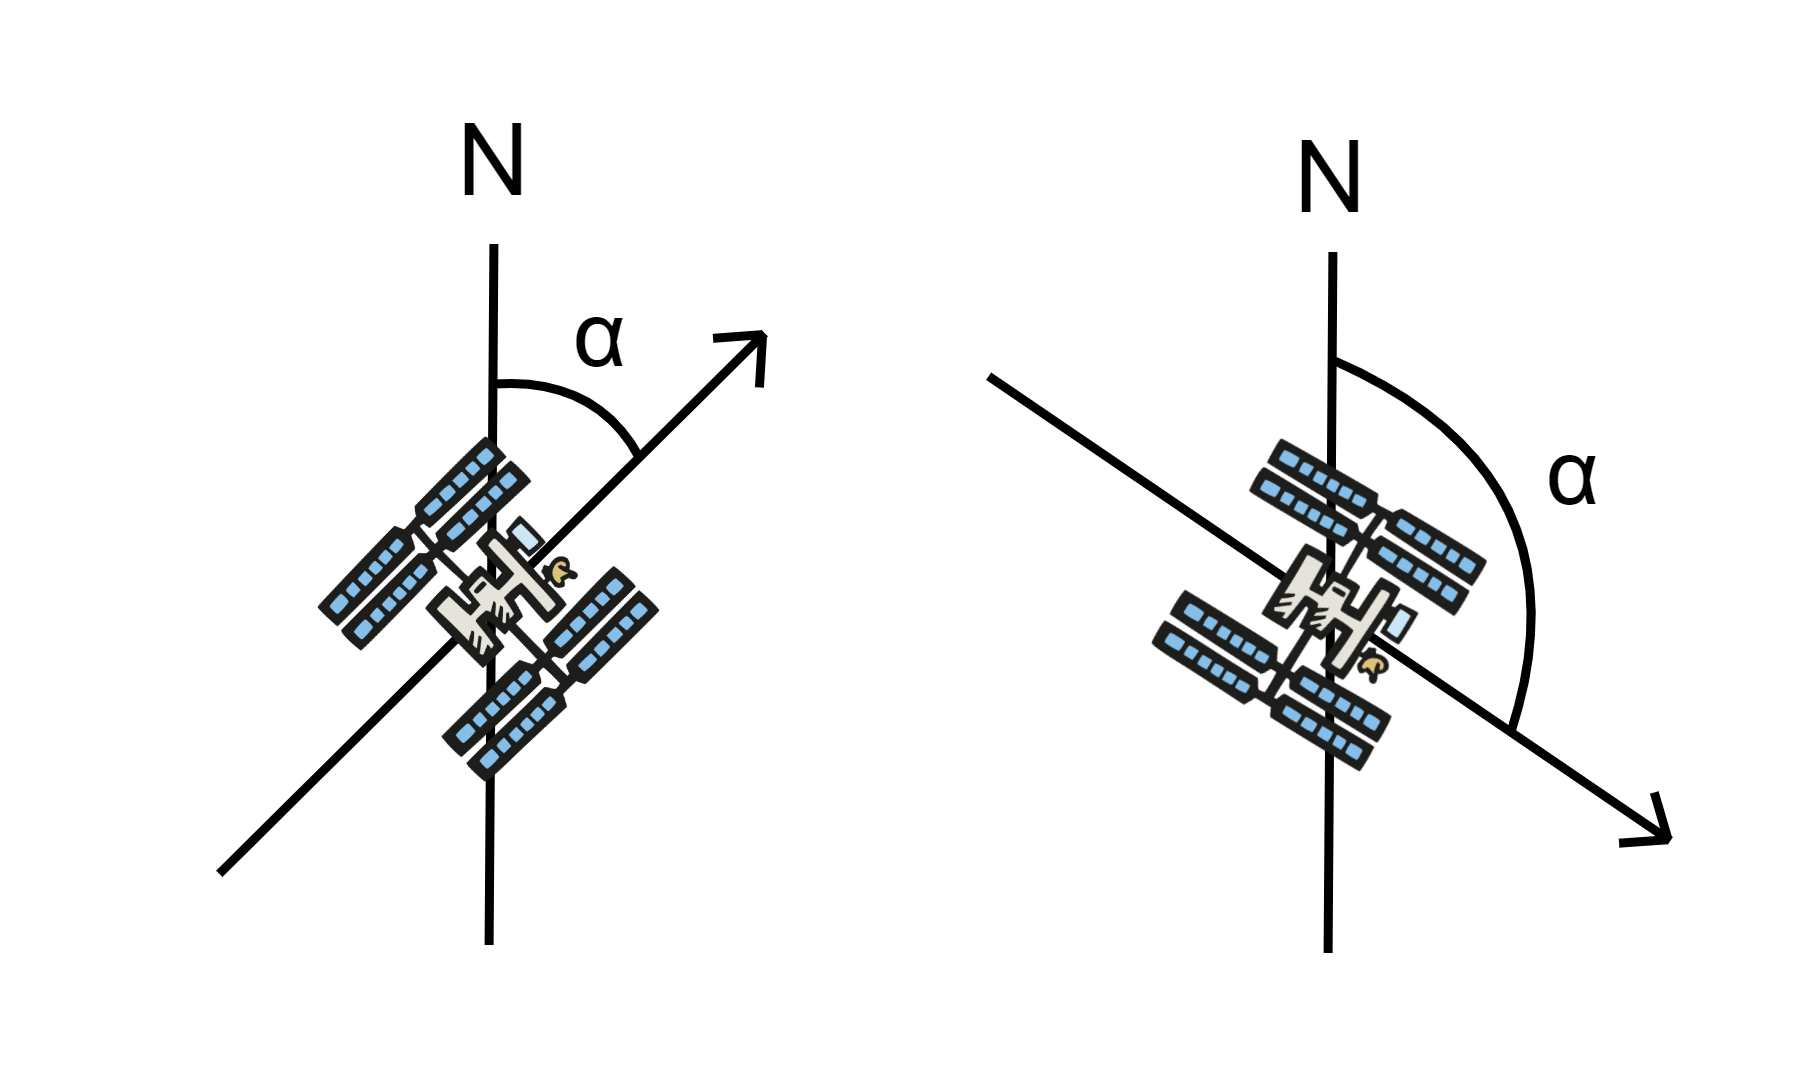
\includegraphics[width=0.8\textwidth]{images/alpha.png}
        \end{center}
        \begin{itemize}
            \item směr pohybu na fotce $\rightarrow$ směr severu z finální rovnice $\rightarrow$ směr stínu z azimutu Slunce 
        \end{itemize}
\end{frame}

\begin{frame}{OpenCV: natočení kamery}
    \begin{columns}[T]
        \begin{column}{.7\textwidth}
            \begin{itemize}
                \item fotka může být \alert{pootočená} 
            \end{itemize}
            \begin{center}
                
\includegraphics[width=0.4\textwidth]{images/open_sever.jpg}
                \vspace{1cm}
                
\includegraphics[width=0.4\textwidth]{images/opencv_pohyb.jpg}
                
\includegraphics[width=0.4\textwidth]{images/opencv_random.jpg}
            \end{center}
        \end{column}
        \begin{column}{.3\textwidth}
            \begin{center}
                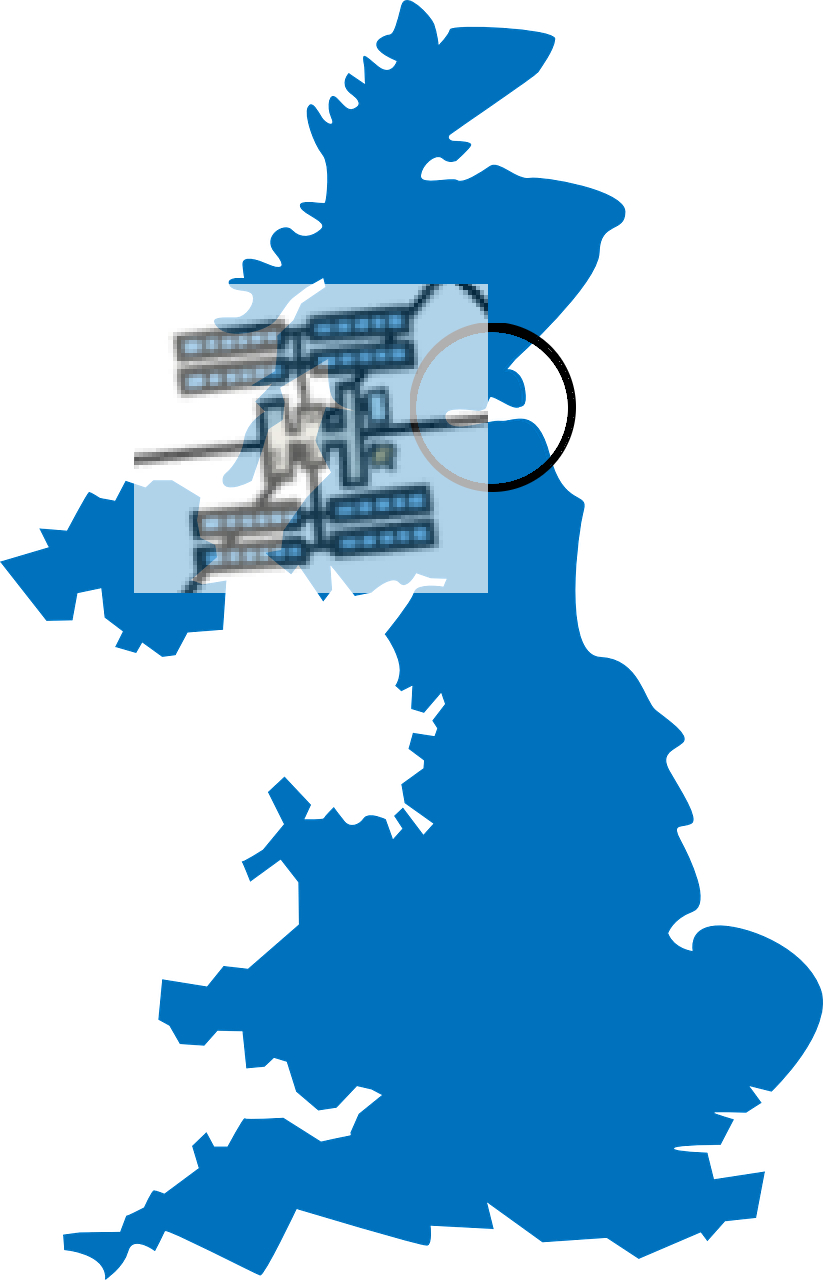
\includegraphics[width=1\textwidth]{images/opencv_britanieISS.jpg}  
            \end{center}
        \end{column}
    \end{columns}
\end{frame}


\begin{frame}{OpenCV: knihovna}
    \begin{itemize}
        \item knihovna pro \alert{manipulaci s obrazem}
        \begin{itemize}
            \item rozpoznávání obličejů
            \item identifikace objektů
            \item klasifikaci lidských akcí ve videu
            \item mnoho dalších...
        \end{itemize} 
    \end{itemize}
    \begin{center}
        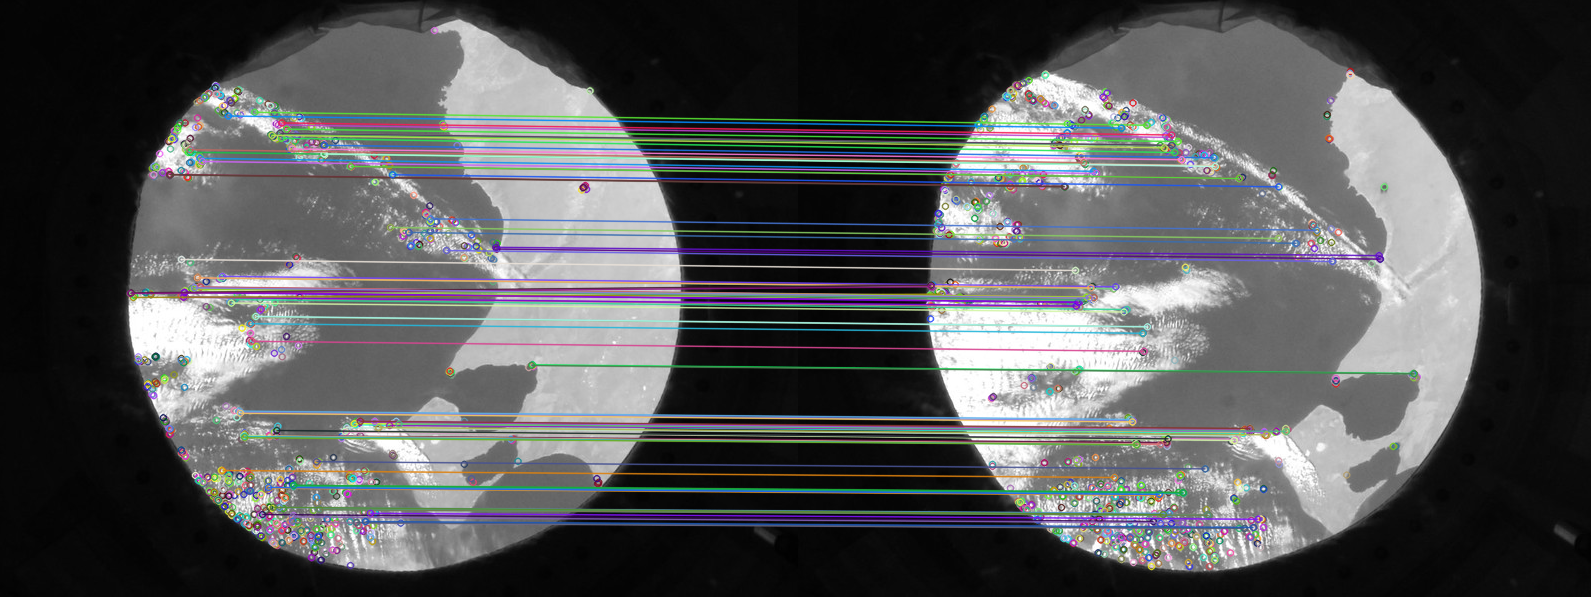
\includegraphics[width=0.9\textwidth]{images/opencv_ukazka.png}
    \end{center}
\end{frame}
            
\begin{frame}{OpenCV: posun obrazu}
        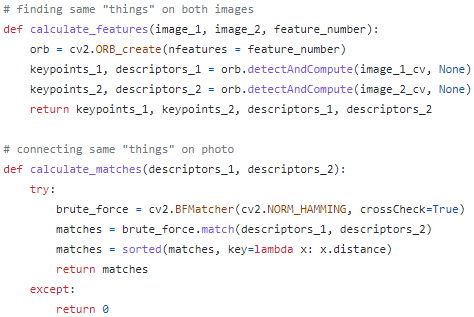
\includegraphics[width=0.8\textwidth]{images/opencv_kod.png}  
  
    \begin{itemize}
                \item z posunu obrazu lze zjistit \alert{natočení kamery}
            \end{itemize}
\end{frame}

\begin{frame}{OpenCV a Sever vůči ISS}
    \begin{itemize}
        \item zkombinováním \alert{polohy severu vůči ISS} a \alert{natočení} kamery získáme \alert{skutečnou polohu severu} na fotce
    \end{itemize}
    \vspace{0.4cm}
        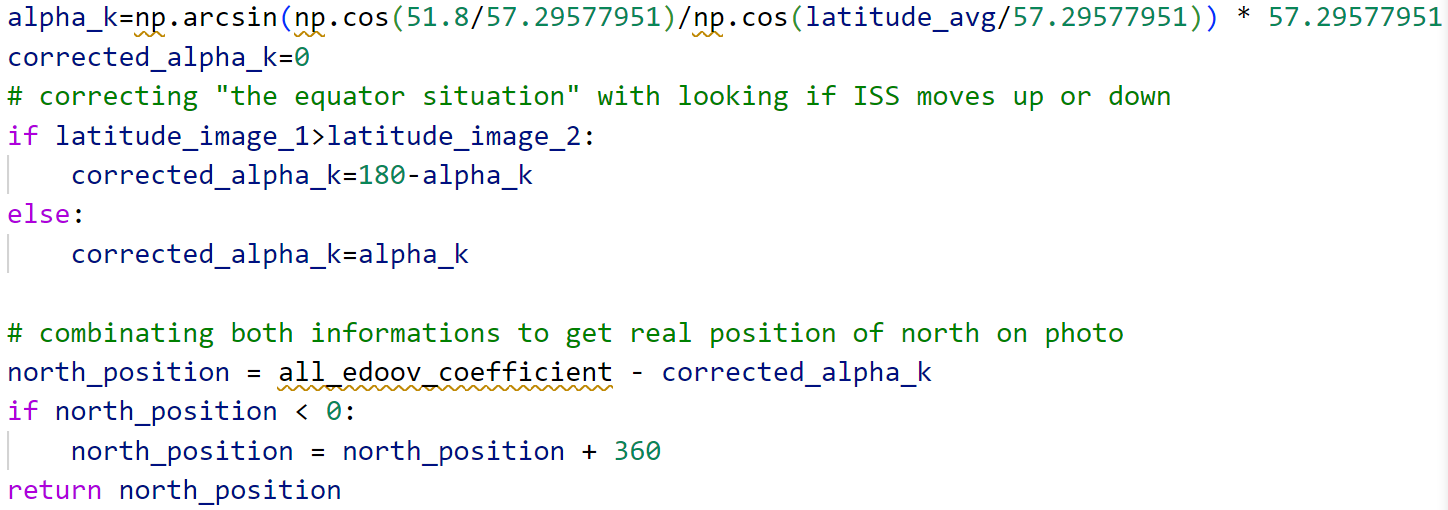
\includegraphics[width=0.9\textwidth]{images/opencv_finalkod.png}
\end{frame}




\begin{frame}[c]
    \begin{center}
    \color{mubeamer@base}
    \huge{\textbf{Jak jsme program implementovali?}}
    \vspace{5mm}
    \Large Praktická ukázka kódu třídy \texttt{north}
    \end{center}
\end{frame}

\subsection[class \texttt{shadow}]{Dlouhý název podsekce 1}
\begin{frame}[c]
\begin{center}
\color{mubeamer@base}
\Huge \textbf{Jak detekovat stíny?}
\end{center}
\end{frame}

\begin{frame}{Jak projet jednotlivé pixely?}
     \begin{columns}[T]
        \begin{column}{.4\textwidth}
        \begin{enumerate}
            \item vypočteme střed mraku podle dat z třídy \texttt{ai} 
        \end{enumerate}
        \end{column}
        \begin{column}{.5\textwidth}
        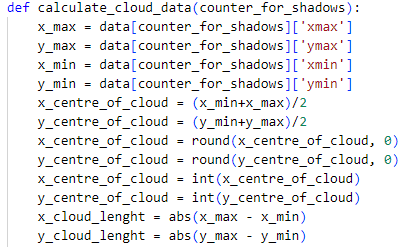
\includegraphics[width =\textwidth] {images/snippet_1.png}
        \end{column}
    \end{columns}
\end{frame}

\begin{frame}{Jak projet jednotlivé pixely?}
     \begin{columns}[T]
        \begin{column}{.4\textwidth}
        \begin{enumerate}
            \setcounter{enumi}{1}
            \item rozdělíme informaci o úhlu na kvadrant a základní úhel 
        \end{enumerate}
        \begin{alertblock}{Směr kvadrantu a úhlu}
          Úhel je počítán po směru hodinových ručiček od severu (i.e. od vrchní strany), kvadranty jsou definovány obdobně, je to tedy jinak než je běžná matematická definice.
        \end{alertblock}
        \end{column}
        \begin{column}{.5\textwidth}
        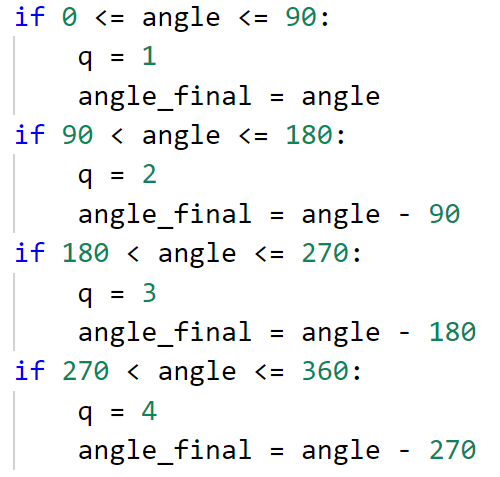
\includegraphics[width =\textwidth]{images/snippet_2.png}
        \end{column}
    \end{columns}
\end{frame}

\begin{frame}{Jak projet jednotlivé pixely?}
     \begin{columns}[T]
        \begin{column}{.4\textwidth}
        \begin{enumerate}
            \setcounter{enumi}{2}
            \item úhel přepočteme na přírůstek $x$ a přírůstek $y$
        \end{enumerate}
        \begin{itemize}
            \item $\alpha = 22.5^{\circ}$ \\ \texttt{x += 0.38} \\ \texttt{y += 0.92}
        \end{itemize}
        \end{column}
        \begin{column}{.5\textwidth}
        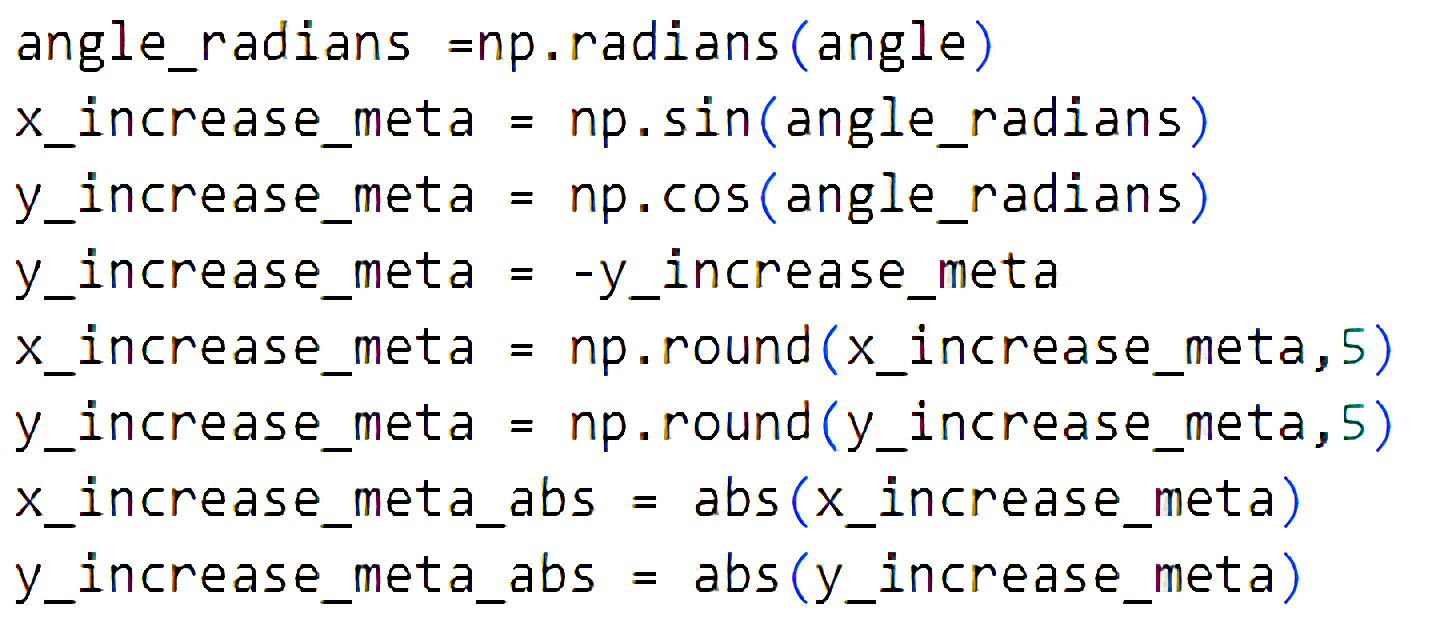
\includegraphics[width =\textwidth]{images/snippet_3(UpRGB)(noise_scale)(Level3)(x4.000000).png}
        \end{column}
    \end{columns}
\end{frame}

\begin{frame}{Jak projet jednotlivé pixely?}
     \begin{columns}[T]
        \begin{column}{.5\textwidth}
        \begin{enumerate}
            \setcounter{enumi}{3}
            \item přírůstky přepočteme tak, aby alespoň jeden z nich byl 1
        \end{enumerate}
        \begin{itemize}
            \item \texttt{x += 0.38}, \texttt{y += 0.87}
            \item \texttt{x += 0.41}, \texttt{y += 1}
        \end{itemize}
        \end{column}
        \begin{column}{.4\textwidth}
          \hspace{3cm}\href{run:./animace.mp4}{(animace)}
        \end{column}
    \end{columns}
    \begin{center}
        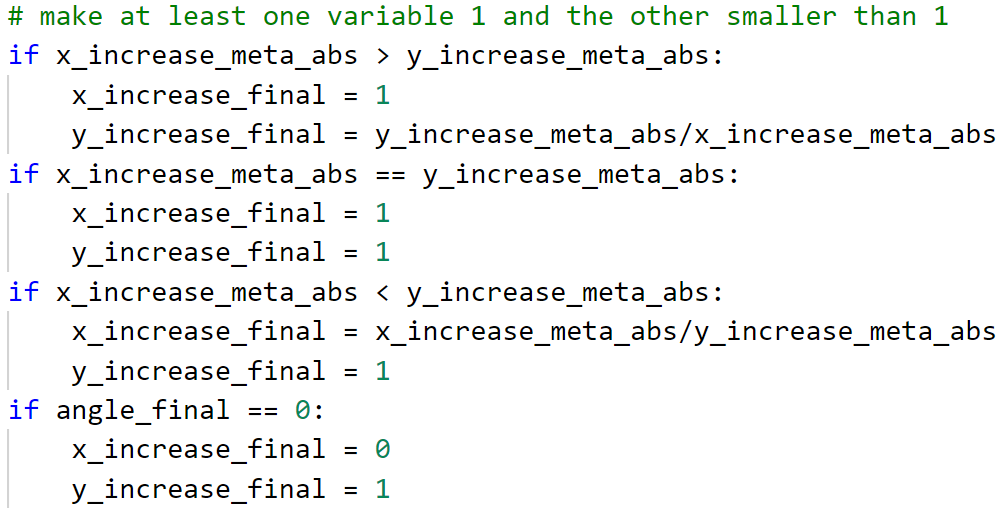
\includegraphics[width = 0.7\textwidth]{images/snippet_4.png}
    \end{center}
\end{frame}

\begin{frame}{Jak projet jednotlivé pixely?}
    \begin{enumerate}
        \setcounter{enumi}{4}
        \item vypočteme tzv. limit hledání stínů
    \end{enumerate}
    \vspace{1cm}
    \begin{center}
        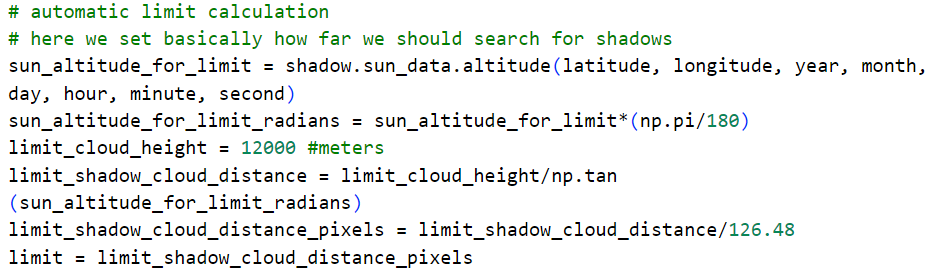
\includegraphics[width = 1\textwidth]{images/snippet_limit.png}
    \end{center}
\end{frame}

\subsection[class \texttt{shadow.sun\_data}]{Dlouhý název podsekce 1}
\begin{frame}{Jak funguje třída \texttt{sun\_data}?}
\begin{center}
    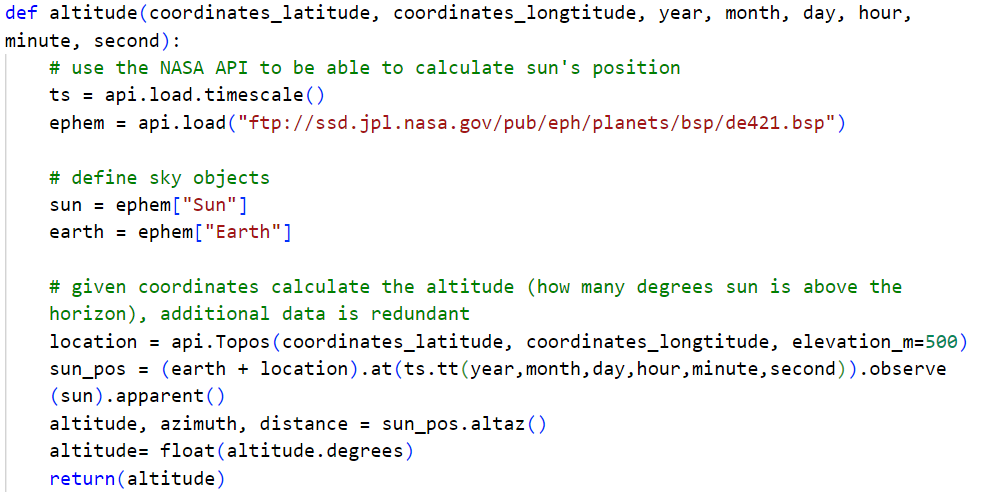
\includegraphics[width = \textwidth]{images/snippet_sundata.png}
\end{center}
\end{frame}

\subsection[class \texttt{shadow}]{Dlouhý název podsekce 1}
\begin{frame}{Jak projet jednotlivé pixely?}
     \begin{columns}[T]
        \begin{column}{.45\textwidth}
            \begin{itemize}
                \item pro každý sektor je loop\footnotemark[13] definován znova
                \item máme tři situace, $x>y$, $x=y$ a $x<y$
                \item celkem máme 12 (4 sektory, 3 situace) možností, jak kód může běžet
                \item kvůli komplikacím s univerzálním řešením jsme nakonec definovali každou situaci zvlášť
            \end{itemize}
        \end{column}
        \begin{column}{.45\textwidth}
        \vspace{-5mm}
        \hspace{-5mm}
        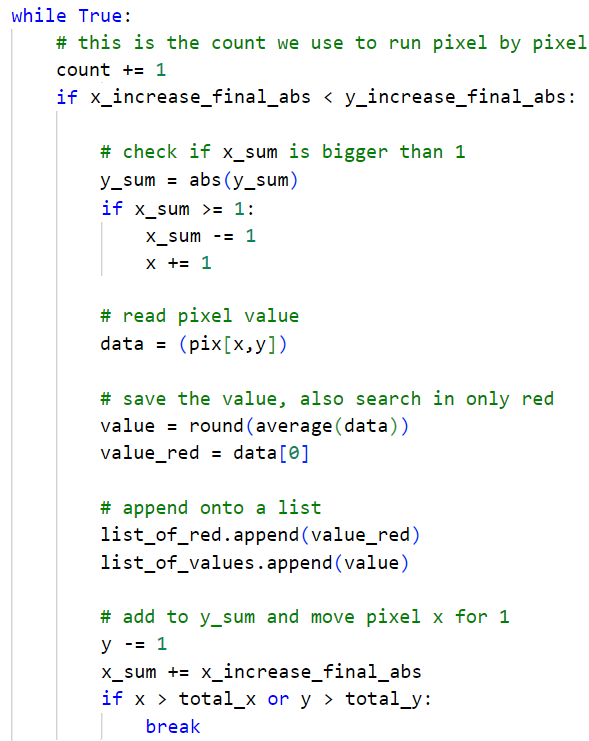
\includegraphics[width=1.1\textwidth]{images/snippet_loop.png}
        \end{column}
    \end{columns}
    \footnotetext[13]{smyčka, běží dokud je podmínka platná}
\end{frame}

\begin{frame}{Jaký je výsledek?}
     \begin{columns}[T]
        \begin{column}{.45\textwidth}
            \begin{itemize}
                \item získáme list obsahující jednotlivé průměrné hodnoty pixelů
                \item a také list obsahující hodnoty jen v červeném spektru
                \item ty poté dále vložíme do jednotlivých funkcí na výpočet vzdálenosti mezi stínem a mrakem
            \end{itemize}
        \end{column}
        \begin{column}{.45\textwidth}
        \texttt{[153, 146, 145, 143, 157, 192, 221, 228, 233, 241, 236, 230, 208, 193, 182, 173, 165, 155, 153, 155, 151, 147, 142, 140, 138, 139, 140, 139, 138, 138, 130, 119, 115, 103, 100, 098, 097, 099, 100, 098, 099, 113, 117, 123, 127, 134, 140, 144]}
        \end{column}
    \end{columns}
\end{frame}

\begin{frame}{Metoda první: minimum-maximum}
     \begin{columns}[T]
        \begin{column}{.45\textwidth}
            \begin{itemize}
                \item v listu najdeme nejvyšší a nejnižší hodnotu
                \item zjistíme pozice těchto hodnot v listu
                \item vypočteme vzdálenost mezi stínem a mrakem
            \end{itemize}
        \end{column}
        \begin{column}{.45\textwidth}
        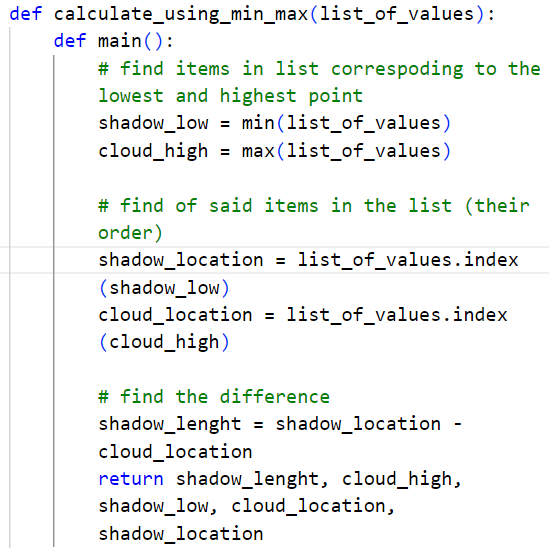
\includegraphics[width=1.0\textwidth]{images/snippet_minmax.png}
        \end{column}
    \end{columns}
\end{frame}

\begin{frame}{Metoda první: minimum-maximum}
     \begin{columns}[T]
        \begin{column}{.45\textwidth}
            \begin{itemize}
                \item když získáme záporný výsledek, stín je před mrakem
                \item tento pixel můžeme smazat - neovlivní to vzdálenost mezi skutečným stínem a mrakem
                \item opakujeme dokud nám nevyjde kladný výsledek
            \end{itemize}
        \end{column}
        \begin{column}{.5\textwidth}
        \includegraphics[width=1.0\textwidth]{images/snippet_minmax_main.png}
        \end{column}
    \end{columns}
\end{frame}

\begin{frame}{Metoda druhá: maximum-change}
     \begin{columns}[T]
        \begin{column}{.45\textwidth}
            \begin{itemize}
                \item nejprve data překonvertujeme na změny
                \item i.e. první derivativ původní funkce
                \item odečteme od sebe sousedící pixely a dáme do nového listu
            \end{itemize}
        \end{column}
        \begin{column}{.45\textwidth}
        \includegraphics[width=1.0\textwidth]{images/snippet_change_convert.png}
        \end{column}
    \end{columns}
\end{frame}

\begin{frame}{Metoda druhá: maximum-change}
     \begin{columns}[T]
        \begin{column}{.45\textwidth}
            \begin{itemize}
                \item poté opět zjistíme umístění těchto hodnot v listu
                \item podle pozice opět vypočteme vzdálenost mezi stínem a mrakem
            \end{itemize}
        \end{column}
        \begin{column}{.45\textwidth}
        \includegraphics[width=1.0\textwidth]{images/snippet_change_search.png}
        \end{column}
    \end{columns}
\end{frame}

\begin{frame}{Metoda druhá: maximum-change}
     \begin{columns}[T]
        \begin{column}{.45\textwidth}
            \begin{itemize}
                \item nakonec opět přidáme ochranu proti záporným výsledkům
                \item smyčka běží, dokud není výsledek kladný
                \item začneme v listu hledat až na pozici 10, aby nedošlo k chybě, kdy \alert{nejvyšší nárůst není způsoben stínem ale mrakem}
            \end{itemize}
        \end{column}
        \begin{column}{.45\textwidth}
        \includegraphics[width=1.0\textwidth]{images/snippet_change_search.png}
        \end{column}
    \end{columns}
\end{frame}

\begin{frame}{Jak vypadá výsledek v grafu?}
\begin{center}
    \includegraphics[width=\textwidth]{images/chart (34).png}
\end{center}
\end{frame}

\begin{frame}{Zprůměrování metod}
     \begin{columns}[T]
        \begin{column}{.45\textwidth}
            \begin{itemize}
                \item nyní máme definované všechny potřebné funkce a metody
                \item využijeme tři výsledky
                \begin{itemize}
                    \item max-change na průměru
                    \item max-change v červené
                    \item min-max na průměru
                \end{itemize}
                \item metody zprůměrujeme
                \item tím získáme vzdálenost mezi stínem a mrakem
                \item délku z pixelů převedeme na metry pomocí konstanty
            \end{itemize}
        \end{column}
        \begin{column}{.5\textwidth}
        \includegraphics[width=1.0\textwidth]{images/snippet_methods_together.png}
        \end{column}
    \end{columns}
\end{frame}

\begin{frame}{Korekce výsledku}
     \begin{columns}[T]
        \begin{column}{.45\textwidth}
            \begin{itemize}
                \item vypočtenou délku je třeba přepočítat z odvěsny na přeponu
                \item jak je vidět v \href{run:./animace.mp4}{(animaci)}, počet pixelů odpovídá delší odvěsně, nikoliv přeponě
                \item výpočet jsou prosté goniometrické funkce
            \end{itemize}
        \end{column}
        \begin{column}{.5\textwidth}
        \includegraphics[width=1.0\textwidth]{images/snippet_correction.png}
        \end{column}
    \end{columns}
\end{frame}

\begin{frame}{Finalizace výsledku}
     \begin{columns}[T]
        \begin{column}{.45\textwidth}
            \begin{itemize}
                \item pomocí již zmíněné rovnice $h = \tan{\alpha}\cdot s$ vypočteme výšku mraku
                \item ještě předtím pomocí třídy \texttt{sun\_data} zjistíme výšku Slunce nad obzorem (i.e. alfa)
                \item výsledek \texttt{shadow\_lenght}, který jsme doposud počítali v rovnici odpovídá $s$
            \end{itemize}
        \end{column}
        \begin{column}{.5\textwidth}
        \includegraphics[width=1.0\textwidth]{images/snippet_final.png}
        \end{column}
    \end{columns}
\end{frame}

\begin{frame}[c]
    \begin{center}
    \color{mubeamer@base}
    \huge{\textbf{Jak jsme program implementovali?}}
    \vspace{5mm}
    \Large Praktická ukázka kódu třídy \texttt{shadow}
    \end{center}
\end{frame}

\section{\bibname}
\begin{frame}[t, allowframebreaks]{\bibname}
\printbibliography[heading=none]
\end{frame}

\begin{frame}[plain]
\vfill
\centerline{Děkuji vám za pozornost!}
\vfill\vfill
\end{frame}

\makeoutro

\end{document}
